\documentclass[12pt]{article}

\usepackage[utf8]{inputenc}
%\usepackage[T1]{fontenc}

\usepackage{geometry}
\geometry{a4paper}
\usepackage{graphicx}
\usepackage{float}
\usepackage[italian]{babel}
\usepackage{listings}
\usepackage{xcolor}
\usepackage{url}
\usepackage{hyperref}
\usepackage{enumitem}


\definecolor{codegreen}{rgb}{0,0.6,0}
\definecolor{codegray}{rgb}{0.5,0.5,0.5}
\definecolor{codepurple}{rgb}{0.58,0,0.82}
\definecolor{backcolour}{rgb}{0.95,0.95,0.92}

\lstdefinestyle{mystyle}{
    backgroundcolor=\color{backcolour},   
    commentstyle=\color{codegreen},
    keywordstyle=\color{magenta},
    numberstyle=\tiny\color{codegray},
    stringstyle=\color{codepurple},
    basicstyle=\ttfamily\footnotesize,
    breakatwhitespace=false,         
    breaklines=true,                 
    captionpos=b,                    
    keepspaces=true,                 
    numbers=left,                    
    numbersep=5pt,                  
    showspaces=false,                
    showstringspaces=false,
    showtabs=false,                  
    tabsize=2
}

% \begin{tabularx}{0.8\textwidth} { 
%   | >{\raggedright\arraybackslash}X 
%   | >{\centering\arraybackslash}X 
%   | >{\raggedleft\arraybackslash}X | }
%  \hline
%  item 11 & item 12 & item 13 \\
%  \hline
%  item 21  & item 22  & item 23  \\
% \hline
% \end{tabularx}
%\usepackage[T1]{fontenc}


% version
\newcommand{\versionmajor}{0}
\newcommand{\versionminor}{1}
\newcommand{\versionpatch}{2}
\newcommand{\version}{\versionmajor.\versionminor.\versionpatch}
\typeout{Document version: \version}



\linespread{1.2}
\setlength{\parindent}{0pt}

\begin{document}

%----------------------------------------------------------------------------------------
%	TITOLO
%----------------------------------------------------------------------------------------

\begin{titlepage}

  \newcommand{\HRule}{\rule{\linewidth}{0.5mm}}

  \center

  \textsc{\Large Relazione di progetto di "Smart City e Tecnologie Mobili"}\\[0.5cm]

  \HRule \\[0.4cm]
  { \huge \bfseries Smart Charging Stations}\\[0.4cm]
  \HRule \\[1.5cm]

  \vfill

  \begin{flushleft}
    \emph{Numero del gruppo: 127}\\[1cm]
    \emph{Componenti del gruppo:\\Cortecchia Angela\\Micelli Leonardo}\\[3cm]

  \end{flushleft}


\end{titlepage}

%----------------------------------------------------------------------------------------
%	INDICE
%----------------------------------------------------------------------------------------

\tableofcontents

\newpage




%----------------------------------------------------------------------------------------
%	INTRODUZIONE
%----------------------------------------------------------------------------------------

\section{Introduzione}
La mobilità elettrica sta rapidamente prendendo piede nelle varie nazioni europee, in particolare nelle grandi città,
dove la necessità di ridurre l'inquinamento atmosferico e acustico è sempre più sentita.

Con un aumento costante nella vendita di veicoli elettrici, la necessità di una rete
di stazioni di ricarica efficienti e ben gestite è diventata cruciale. Tuttavia,
il crescente numero di veicoli elettrici nelle strade presenta sfide uniche per la loro gestione.

La disponibilità delle stazioni di ricarica e la loro efficienza possono influenzare
significativamente l'esperienza degli utenti e il successo complessivo della mobilità elettrica.

È in questo contesto che il progetto \textit{"Smart Charging Stations"} prende vita. Si mira a
fornire una soluzione completa e avanzata per la gestione delle stazioni di ricarica, con
l'obiettivo di semplificare il processo di ricarica per gli utenti e promuovere una mobilità sostenibile.
\subsection{Obiettivo del progetto}
L'obiettivo primario del progetto \textit{"Smart Charging Stations"} è migliorare l'esperienza della
mobilità elettrica nelle smart cities attraverso l'implementazione di un sistema di gestione avanzato
per le stazioni di ricarica dei veicoli elettrici. Questa soluzione tecnologica mira a semplificare e
ottimizzare l'utilizzo delle stazioni di ricarica, fornendo agli utenti un accesso facile, rapido ed
efficiente alle risorse di ricarica, contribuendo così alla diffusione su larga scala dei veicoli elettrici
e alla promozione di una mobilità sostenibile.

\subsection{Caratteristiche salienti}
Il progetto \textit{"Smart Charging Stations"} si distingue per diverse caratteristiche salienti.

Dal punto di vista dell'utente, l'applicazione sviluppata permetterà di individuare facilmente le
stazioni di ricarica disponibili all'interno della smart city attraverso una mappa interattiva, permettendo anche di
salvare dei punti di interesse.
Questa funzionalità si basa sull'integrazione di tecnologie di geolocalizzazione per applicativi web.

Un altro elemento chiave è la visualizzazione dello stato delle stazioni di ricarica.
Gli utenti potranno vedere in tempo reale se una stazione è occupata, prenotata o libera, permettendo
agli utenti di pianificare la loro sosta prenotando una stazione in anticipo, eliminando la frustrazione di arrivare a una stazione
solo per trovarla occupata.

Inoltre, l'applicazione permetterà di sbloccare le stazioni di ricarica tramite QR code, garantendo un accesso sicuro e veloce alle risorse di ricarica.

\subsection{Contributo tecnologico-scientifico apportato}
Il contributo maggiore che il progetto \textit{"Smart Charging Stations"} ha apportato
è senza dubbio nel campo dello studio di architetture distribuite per tecnologie per smart
cities.

In particolare, esso ha riguardato la progettazione di un'architettura semi-decentralizzata
e l'ottimizzazione dei flussi di dati all'interno del sistema.\\

Ciò è stato possibile grazie all'impiego di tecnologie per l'implementazione di sistemi
altamente concorrenti, come Scala \cite{scala} e Akka\cite{akka}, grazie alle quali è
stato sviluppato il core decentralizzato del sistema.
Ad esse sono state integrate tecnologie web per lo sviluppo di web app, come JavaScript\cite{javascript}
e Svelte\cite{svelte}, e per il deployment di servizi web come Nodejs\cite{node} e MongoDB\cite{mongo}.\\

In conclusione, il progetto \textit{"Smart Charging Stations"} rappresenta il tentativo di
effettuare un passo avanti verso una mobilità elettrica più efficiente e accessibile
nelle smart cities.\\

Grazie alle tecnologie integrate, all'interfaccia intuitiva e alle funzionalità
avanzate, ci proponiamo di favorire l'adozione su larga scala dei veicoli elettrici,
contribuendo così a un futuro più sostenibile e intelligente.


% =====================================================
%Esporre l’obiettivo del progetto dandone una visione complessiva.\\

%Devono essere illustrate le caratteristiche salienti del progetto; deve essere chiara la distinzione tra le tecnologie usate/assemblate durante lo svolgimento dell'elaborato e il contributo tecnologico/scientifico effettivamente apportato dal gruppo.\\


% Vincoli circa la lunghezza della sezione (escluse didascalie, tabelle, testo nelle immagini, schemi):

% \vspace{1cm}
% \begin{tabular}{l|rr}
%                  & Numero minimo di battute & Numero massimo di battute \\
%     \hline
%     1 componente & 2000                     & 3000                      \\
%     2 componenti & 2500                     & 4500                      \\
%     3 componenti & 3000                     & 6000                      \\
%     \hline
% \end{tabular}


\newpage


%----------------------------------------------------------------------------------------
%	STATO DELL'ARTE
%----------------------------------------------------------------------------------------

\section{Stato dell'arte}

Attualmente, le soluzioni che offrono esperienze simili a quella sviluppata nella nostra app possono essere categorizzate
come applicazioni di navigazione, come ad esempio Google Maps.
Queste applicazioni permettono agli utenti di cercare stazioni di ricarica per veicoli elettrici nel territorio
limitrofo e, conseguentemente, di pianificare un percorso che includa una o più soste per la ricarica.\\

Un problema che questo sistema può causare è che non si conosce lo stato attuale delle colonnine. Di conseguenza,
potrebbe accadere che si crei un itinerario che includa una stazione di ricarica occupata o non funzionante,
causando problemi e ritardi all'utente.\\

Inoltre, le stazioni di ricarica stanno diventando parte integrante delle reti intelligenti delle città,
contribuendo alla creazione di ecosistemi di mobilità sostenibile. Questo significa che in futuro potremmo
vedere un aumento delle stazioni di ricarica interoperabili, accessibili tramite una varietà di fornitori
e gestite centralmente attraverso piattaforme unificate.\\

L'idea alla base del progetto in esame trae ispirazione da queste evoluzioni del settore. Si sta cercando
di anticipare le esigenze degli utenti, offrendo un'applicazione che non solo consente di trovare stazioni
di ricarica, ma fornisce anche informazioni in tempo reale sull'occupazione delle colonnine. Inoltre, si sta
lavorando per garantire che l'applicazione sia compatibile con una varietà di fornitori di stazioni di ricarica,
offrendo agli utenti una scelta più ampia e la possibilità di pianificare itinerari ottimizzati.\\

L'idea per lo sviluppo di questo progetto ha tratto ispirazione dall'applicazione MooneyGo (ex MyCicero). Tuttavia,
questa app non fornisce questo tipo di servizio ma consente di pagare parcheggi o ticket per i mezzi pubblici
tramite smartphone, inclusi biciclette e monopattini elettrici, che sono localizzabili attraverso l'applicazione.\\

Il concetto iniziale del progetto è nato considerando che un servizio di questo tipo potrebbe essere esteso anche
alle stazioni di ricarica per veicoli elettrici. In un contesto urbano di medie o grandi dimensioni, è possibile
che un utente debba spostarsi in auto per svolgere delle commissioni. Pertanto, sarebbe vantaggioso se l'utente
potesse sfruttare al meglio il tempo trascorso durante la sosta, ricaricando il proprio veicolo.\\


Un altro esempio di applicazione presente sul mercato è quella di un provider energetico come Enel X.
Questa app consente agli utenti di localizzare le colonnine di ricarica e di effettuare il pagamento della
ricarica direttamente tramite l'applicazione. Tuttavia, presenta alcune limitazioni. Innanzitutto,
è specifica del provider Enel X, il che significa che mostra solo le colonnine di ricarica appartenenti
a questo provider. Questo può essere un inconveniente per gli utenti che desiderano avere una scelta più
ampia di stazioni di ricarica, tenendo conto di fattori come i costi e i percorsi più convenienti per il proprio itinerario.\\

Inoltre, un'altra sfida con cui gli utenti si possono confrontare è la mancanza di informazioni in tempo
reale sullo stato delle stazioni. Nonostante l'app permetta di localizzare le stazioni, gli utenti potrebbero
non sapere se una di esse è attualmente occupata o disponibile. Questa mancanza di informazioni aggiornate
potrebbe portare a situazioni in cui gli utenti arrivano alla stazione di ricarica solo per scoprire che è
occupata, causando disagi e ritardi.

% =============================================

% Riassumere le soluzioni presenti in letteratura inerenti al problema in esame. Per ciascuna, discutere le principali diversità o affinità rispetto al progetto presentato. Nel caso non siano presenti soluzioni direttamente comparabili a quella presentata descrivere comunque le principali tecniche note per affrontare la tematica trattata.\\

% Le soluzioni esposte devono essere corredate degli opportuni riferimenti bibliografici. Nel caso si tratti di soluzioni già operative sul mercato, devono essere indicate le fonti (online) dove poter accedere al servizio o approfondirne i contenuti.\\


% Vincoli circa la lunghezza della sezione (escluse didascalie, tabelle, testo nelle immagini, schemi):

% \vspace{1cm}
% \begin{tabular}{l|rr}
%                  & Numero minimo di battute & Numero massimo di battute \\
%     \hline
%     1 componente & 2000                     & 3000                      \\
%     2 componenti & 2500                     & 4500                      \\
%     3 componenti & 3000                     & 6000                      \\
%     \hline
% \end{tabular}


\newpage

%----------------------------------------------------------------------------------------
%	ANALISI DEI REQUISITI
%----------------------------------------------------------------------------------------

\section{Analisi dei requisiti}
In questa sezione, verranno esplicitati dettagliatamente i requisiti del sistema,
suddivisi in diverse categorie precedentemente identificate. Durante la fase di
analisi dei requisiti, è stato adottato un ruolo attivo da stakeholder al fine di
acquisire una comprensione completa delle esigenze degli utenti e influenzare positivamente
lo sviluppo del sistema.\\

Questo approccio ha consentito al team di progettazione di immergersi completamente
nell'ottica degli utilizzatori finali, facilitando l'identificazione precisa delle
azioni principali previste all'interno del sistema. Ciò ha portato alla definizione di requisiti specifici, attentamente elaborati per soddisfare le effettive necessità degli utenti e garantire un'ottimale esperienza utente.\\

In sintesi, è stato svolto un ruolo attivo nell'acquisizione delle esigenze degli
stakeholder, ponendosi nella prospettiva degli utilizzatori finali. Attraverso
questo processo di comprensione approfondita, sono stati delineati requisiti
chiari e dettagliati che servono da guida per lo sviluppo del sistema.

\subsection{Requisiti di Business}
I requisiti aziendali definiscono le ragioni per cui un'organizzazione intraprende un progetto e quali risultati aziendali si prevede di raggiungere attraverso di esso. I requisiti di business sono fondamentali per guidare lo sviluppo di soluzioni software o progetti affinché siano allineati agli obiettivi e alle esigenze dell'azienda.

\begin{enumerate}
    \item Incremento dell'Utilizzo delle Stazioni di Ricarica: L'obiettivo principale è facilitare l'utilizzo delle stazioni di ricarica per veicoli elettrici, rendendole più accessibili e convenienti per gli utenti.

    \item Migliorare l'Esperienza dell'Utente: L'esperienza dell'utente è una priorità, con l'obiettivo di semplificare il processo di ricerca e utilizzo delle stazioni di ricarica, riducendo le frustrazioni legate alla disponibilità e alla gestione delle stazioni.

    \item Promuovere la Sostenibilità Ambientale: L'applicazione si impegna a promuovere la mobilità elettrica come mezzo per ridurre l'inquinamento atmosferico nelle città, contribuendo alla sostenibilità ambientale.

    \item Integrazione nelle Smart Cities: L'applicazione cerca di integrarsi in un contesto di smart city, migliorando l'efficienza dei trasporti urbani e la qualità della vita urbana.
\end{enumerate}

\subsection{Requisiti utente}
I requisiti utente sono focalizzati sull'esperienza dell'utente finale e su come essi interagiranno con il sistema.

Per delineare le azioni principali che un utente può compiere all'interno dell'applicazione, sono stati studiati vari scenari d'uso.
Per facilitarne la comprensione e la visualizzazione, è stato creato un diagramma dei casi d'uso (figura \ref{fig:casiduso}), che mostra le azioni principali che un utente può compiere all'interno dell'applicazione.
\begin{enumerate}[label=\arabic*.]
    \item Visualizzazione dello stato di una singola stazione di ricarica
          \begin{enumerate}[label=\arabic{enumi}.\arabic*]
              \item Stazione riservata
              \item Stazione libera
              \item Stazione in fase di ricarica
          \end{enumerate}
    \item Visualizzazione di una mappa con le stazioni all'interno del territorio limitrofo
          \begin{enumerate}[label=\arabic{enumi}.\arabic*]
              \item Visualizzazione dello stato (semplificato) di tutte le stazioni
              \item Possibilità di selezionare una stazione nella mappa
              \item Visualizzazione di informazioni dettagliate sulla colonnina
              \item Possibilità di selezionare una stazione nella mappa
          \end{enumerate}
    \item Servizi di autenticazione per l'accesso all'applicazione
          \begin{enumerate}[label=\arabic{enumi}.\arabic*]
              \item Registrazione
              \item Login
          \end{enumerate}
    \item Gestione delle stazioni di ricarica
          \begin{enumerate}[label=\arabic{enumi}.\arabic*]
              \item Prenotazione di una stazione di ricarica
              \item Sblocco di una colonnina con QR code e fotocamera per avviare la ricarica
              \item Aggiunta e rimozione di stazione d'interesse
          \end{enumerate}
    \item Interfacciamento con servizi esterni tramite http
\end{enumerate}

\begin{figure}[htbp]
    \centering
    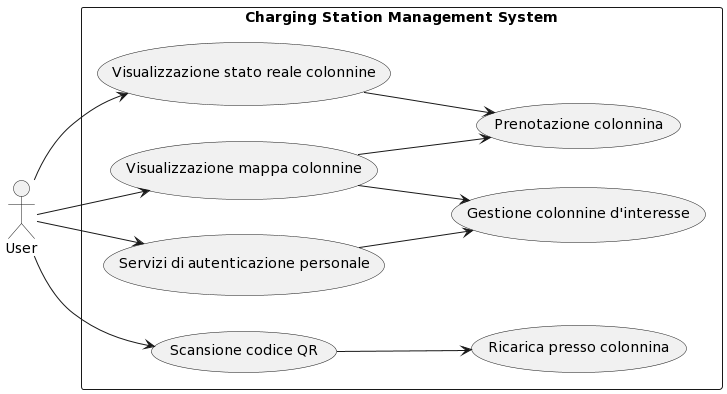
\includegraphics[width=\textwidth]{images/casiduso.png}
    \caption{Diagramma dei Casi d'Uso}
    \label{fig:casiduso}
\end{figure}

\subsection{Requisiti Funzionali}
I requisiti funzionali descrivono le funzionalità specifiche che il sistema deve fornire,
come il sistema deve reagire a determinati input e come deve comportarsi in situazioni specifiche.\\


\begin{enumerate}[label=\arabic*.]
    \item Registrazione Utente
          \begin{enumerate}[label=\arabic{enumi}.\arabic*]
              \item Gli utenti devono poter creare un account fornendo informazioni personali, tra cui nome, cognome, indirizzo email e password.
              \item L'applicazione deve verificare l'unicità dell'indirizzo email.
          \end{enumerate}

    \item Login Utente
          \begin{enumerate}[label=\arabic{enumi}.\arabic*]
              \item Gli utenti registrati devono poter effettuare il login inserendo l'indirizzo email e la password.
          \end{enumerate}

    \item Visualizzazione della Mappa delle Stazioni di Ricarica
          \begin{enumerate}[label=\arabic{enumi}.\arabic*]
              \item Gli utenti devono poter visualizzare la loro posizione all'interno di una mappa, dopo aver acconsentito all'utilizzo di geolocalizzazione.
              \item Gli utenti devono poter visualizzare una mappa interattiva che mostra la posizione delle stazioni di ricarica per veicoli elettrici all'interno del territorio limitrofo.
              \item Le stazioni devono essere rappresentate da icone distintive sulla mappa.
          \end{enumerate}

    \item Visualizzazione dello Stato delle Stazioni
          \begin{enumerate}[label=\arabic{enumi}.\arabic*]
              \item Gli utenti devono poter vedere lo stato di ciascuna stazione di ricarica direttamente sulla mappa. Lo stato può essere "occupata," "libera," o "in fase di ricarica."
              \item Cliccando su una stazione, gli utenti possono ottenere informazioni dettagliate sulla colonnina, incluso l'indirizzo.
          \end{enumerate}

    \item Prenotazione di una Stazione di Ricarica
          \begin{enumerate}[label=\arabic{enumi}.\arabic*]
              \item Gli utenti devono poter prenotare una stazione di ricarica disponibile tramite l'applicazione.
          \end{enumerate}

    \item Sblocco di una Stazione con QR Code
          \begin{enumerate}[label=\arabic{enumi}.\arabic*]
              \item Gli utenti devono poter sbloccare una stazione di ricarica prenotata o libera utilizzando un codice QR posizionato sulla colonnina.
              \item L'applicazione deve poter leggere il codice QR, dopo la richiesta di utilizzo della fotocamera del dispositivo.
          \end{enumerate}

    \item Gestione delle Stazioni d'Interesse
          \begin{enumerate}[label=\arabic{enumi}.\arabic*]
              \item Gli utenti possono aggiungere stazioni di ricarica alla loro lista di "stazioni d'interesse."
              \item Devono poter rimuovere stazioni dalla lista d'interesse in qualsiasi momento.
          \end{enumerate}

    \item Localizzazione
          \begin{enumerate}[label=\arabic{enumi}.\arabic*]
              \item L'applicazione deve supportare servizi di geolocalizzazione in tempo reale.
          \end{enumerate}
\end{enumerate}

\subsection{Requisiti non Funzionali}
I requisiti non funzionali sono criteri e specifiche che definiscono il comportamento complessivo di un sistema software o di un'applicazione, ma non si concentrano direttamente sulle funzionalità principali.

Nel caso di \textit{Smart Charging Stations}:

\begin{enumerate}[label=\arabic*.]
    \item Performance: L'applicazione deve essere altamente performante, consentendo agli utenti di accedere rapidamente alle informazioni sulle stazioni di ricarica e di effettuare prenotazioni senza ritardi significativi.

    \item Usabilità: L'interfaccia utente dell'applicazione deve essere intuitiva e user-friendly, garantendo un'esperienza d'uso piacevole. In particolare, le mappe devono essere facili da navigare, e le operazioni di prenotazione e sblocco delle stazioni devono essere semplici da eseguire.

    \item Disponibilità: Il sistema deve essere disponibile 24/7, in modo che gli utenti possano accedervi in qualsiasi momento per visualizzare le stazioni di ricarica e effettuare prenotazioni.

    \item Compatibilità: L'applicazione deve essere compatibile con una vasta gamma di dispositivi mobili, inclusi smartphone e tablet, e deve funzionare su diverse piattaforme, come iOS e Android.

    \item Scalabilità: Il sistema deve essere progettato per gestire un grande numero di utenti simultanei senza degradazione delle prestazioni.

    \item Manutenzione e Aggiornamenti: Il sistema deve essere facilmente manutenibile e consentire l'aggiornamento regolare per introdurre nuove funzionalità e correzioni di bug.
\end{enumerate}

\subsection{Requisiti di Implementazione}
I requisiti di implementazione sono specifici per il sistema software e definiscono le caratteristiche tecniche che il sistema deve soddisfare.

\begin{enumerate}[label=\arabic*.]
    \item Linguaggio di programmazione: L'applicazione deve essere sviluppata utilizzando il linguaggio di programmazione Scala lato server per gestione delle colonnine, deve utilizzare il framework Express.js lato web server e il linguaggio Svelte per quanto riguarda l'interfaccia utente.
    \item Architettura Orientata agli Attori con Akka HTTP: L'implementazione deve aderire al paradigma basato su attori, sfruttando il framework Akka, incluso Akka HTTP, per gestire l'interazione tra i nodi del sistema.
    \item Tecnologie di Persistenza: La componente responsabile della conservazione dei dati deve essere sviluppata utilizzando MongoDB ed interfacciarsi con il server Node.
\end{enumerate}



% ===============================
% In questa sezione esporre brevemente i requisiti a cui il sistema proposto deve rispondere, concentrando l'attenzione sugli aspetti più rilevanti e facendo eventualmente uso di opportuni diagrammi di alto livello.\\

% Vincoli circa la lunghezza della sezione (escluse didascalie, tabelle, testo nelle immagini, schemi):

% \vspace{1cm}
% \begin{tabular}{l|rr}
%                  & Numero minimo di battute & Numero massimo di battute \\
%     \hline
%     1 componente & 4000                     & 6000                      \\
%     2 componenti & 6000                     & 8000                      \\
%     3 componenti & 8000                     & 10000                     \\
%     \hline
% \end{tabular}


\newpage

%----------------------------------------------------------------------------------------
%	PROGETTAZIONE
%----------------------------------------------------------------------------------------

\section{Progettazione}
Il processo di sviluppo adottato ha visto due fasi di progettazione ben distinte: il design architetturale e il design di dettaglio.\\

\subsection{Design Architetturale}

Dapprima il gruppo si è concentrato sul design architetturale, ovvero la definizione dell'architettura generale del sistema, delle sue componenti principali e delle relazioni tra di esse.\\
Ciò ha permesso di individuare fin da subito gli elementi più importanti del sistema e di definire le interfacce tra di essi, nonchè di scegliere le tecnologie più appropriate
per supportare il core del sistema.\\

Fin dalle prime fasi di analisi sono emersi due domini distinti ma connessi tra di loro:
\begin{itemize}
    \item \textbf{User Domain}: comprende tutti i componenti del sistema che concorrono a fornire un'interfaccia di accesso al sistema all'utente finale.
    \item \textbf{Charging Station Domain}: comprende tutti i componenti del sistema che concorrono a modellare il comportamento delle Charging Station e di monitornarne costantemente lo stato.
\end{itemize}

In seguito all'individuazione di questi domini, il gruppo ha individuato per ognuno di essi le componenti principali, che verranno di seguito discusse. \\

Per quanto riguarda lo User Domain:
\begin{itemize}
    \item \textbf{User App}: applicativo utilizzato dall'utente finale, costituisce l'interfaccia principale con il sistema, permettendo di visualizzare i dati e di interagire con esso.
    \item \textbf{Auth Server}: servizio che permette di registrare ed autenticare gli utenti permettendo loro di accedere al sistema. \\
    \item \textbf{User DB}: database che contiene le informazioni sugli utenti registrati al sistema.
\end{itemize}

La User App, all'avvio, richiederà all'utente di autenticarsi o registrarsi e genererà una richiesta HTTP da inviare all'Auth Server. Quest'ultimo interrogherà il database per verificare l'esistenza
dell'utente o per crearne uno nuovo. In seguito alla riuscita di queste operazioni, l'utente avrà accesso alla User App e potrà interagire con il sistema.\\

Per quanto riguarda il Charging Station Domain:
\begin{itemize}
    \item \textbf{Charging Station}: componente hardware che permette di ricaricare le batterie dei veicoli elettrici.
    \item \textbf{Charging Station Actor}: componente software che gestisce la Charging Station, permettendo di monitorare lo stato della stessa e di interagire con essa.
    \item \textbf{Charging Station Provider}: componente software che osserva lo stato delle Charging Station e ne fornisce un'interfaccia di accesso.
    \item \textbf{Charging Station Service}: sotto componente del Charging Station Provider, permette di esporre l'interfaccia del Charging Station Provider attraverso una API REST. \\
\end{itemize}

Siccome i dati relativi alle Charging Station sono conosciuti ed utilizzati dal Charging Station Actor, il gruppo ha deciso di non creare al momento un Database per memorizzarli, ma di utilizzare un modello a scambio di messaggi per effettuare
query direttamente sui Charging Station Actors.\\

I vari Charging Station Actors dunque gestiscono in maniera indipendente le Charging Station, e comunicano in maniera peer-to-peer con il Charging Station Provider, il quale può sia essere notificato
dai Charging Station Actors di eventuali cambiamenti di stato, sia interrogato dalla User App per ottenere informazioni sullo stato delle Charging Station attraverso l'API REST esposta dal Charging Station Service.\\

L'architettura complessiva del sistema è dunque riassunta nel seguente diagramma:

\begin{figure}[htbp]
    \centering
    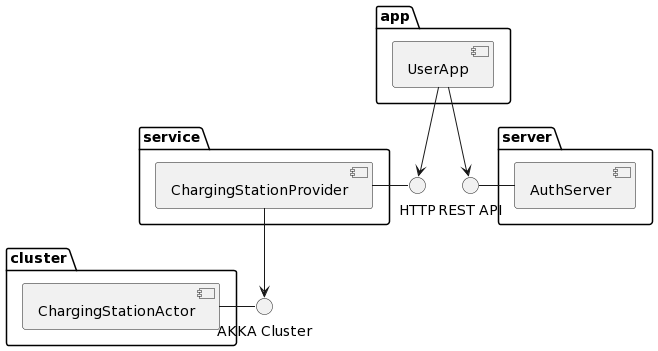
\includegraphics[width=\textwidth]{images/architecture.png}
    \caption{Diagramma dei Componenti per l'architettura del sistema}
    \label{fig:architecture}
\end{figure}

\subsubsection{Interazione tra le componenti del sistema}
Una volta individuate le componenti principali del sistema, il gruppo ha definito le interazioni tra di esse, in modo da poter definire le interfacce di comunicazione tra loro.\\
In seguito saranno riportate le interazioni tra le componenti del sistema, elencate per caso d'uso.\\

\paragraph{Signup di un utente}
L'utente inizia il processo di registrazione nell'applicazione. L'utente interagisce con l'applicazione utente e fornisce un nome utente, un indirizzo email e una password per registrarsi.

L'applicazione utente invia quindi una richiesta di registrazione al servizio di autenticazione. Questo, a sua volta, comunica con un database degli utenti.

Il servizio di autenticazione cerca nel database se l'indirizzo email fornito dall'utente è già presente. In caso negativo esso comunica all'applicazione utente che l'utente è stato registrato con successo, e l'applicazione utente restituisce una risposta positiva all'utente.

Tuttavia, se l'indirizzo email è già presente nel database, il servizio di autenticazione informa l'applicazione utente che l'indirizzo email è già in uso, e l'applicazione utente restituisce una risposta negativa all'utente.

In entrambi i casi, l'applicazione utente fornisce una risposta all'utente per comunicare l'esito della registrazione.

Questa interazione è riassunta nel seguente diagramma di sequenza:
\begin{figure}[htbp]
    \centering
    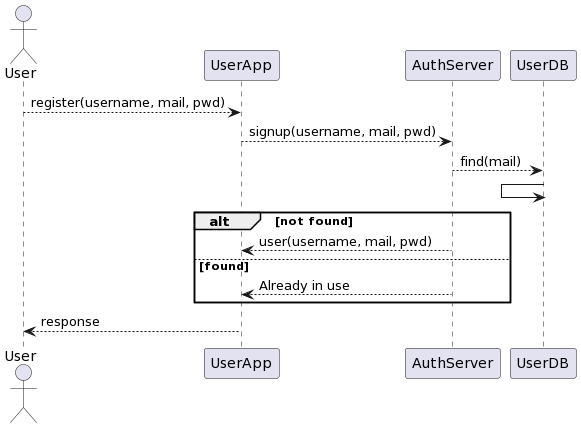
\includegraphics[width=\textwidth]{images/signup.png}
    \caption{Diagramma delle sequenze per la registrazione di un utente}
    \label{fig:signup}
\end{figure}

\paragraph{Login di un utente}
L'utente inizia il processo di accesso (login) nell'applicazione. L'utente interagisce con l'applicazione utente e fornisce il proprio indirizzo email e la password per effettuare l'accesso.

L'applicazione utente invia quindi una richiesta di accesso al Servizio di Autenticazione. Questo servizio comunica con un database degli utenti.

Il Servizio di Autenticazione cerca nel database le credenziali fornite dall'utente per verificare se corrispondono a un account registrato. Se le credenziali sono corrette (caso di successo), il Servizio di Autenticazione comunica all'applicazione utente che l'utente è stato autenticato con successo, e l'applicazione utente restituisce una risposta positiva all'utente.

Tuttavia, se le credenziali fornite non sono corrette (caso di fallimento), il Servizio di Autenticazione informa l'applicazione utente che l'indirizzo email o la password sono errati, e l'applicazione utente restituisce una risposta negativa all'utente.

In entrambi i casi, l'applicazione utente fornisce una risposta all'utente per comunicare l'esito del tentativo di accesso.\\

Questa interazione è riassunta nel seguente diagramma di sequenza:
\begin{figure}[htbp]
    \centering
    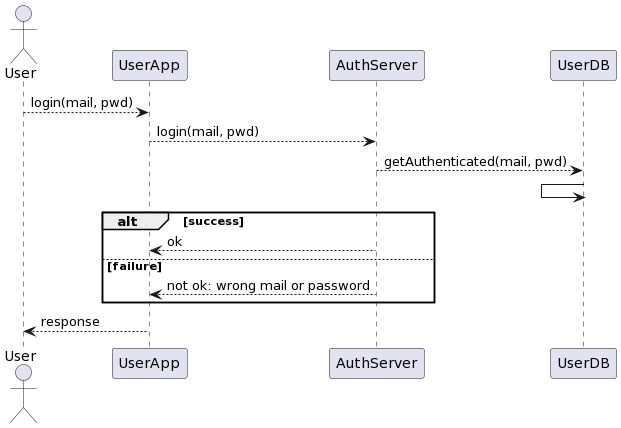
\includegraphics[width=\textwidth]{images/login.png}
    \caption{Diagramma delle sequenze per il login di un utente}
    \label{fig:login}
\end{figure}

\paragraph{Visualizzazione dello stato di una stazione di ricarica}
L'utente interagisce con l'applicazione utente e seleziona una stazione di ricarica.

L'applicazione utente invia quindi una richiesta per ottenere informazioni sulla stazione di ricarica selezionata al Charging Station Service. Questo a sua volta comunica con il Provider.

Il Provider cerca le informazioni sulla stazione di ricarica identificata dall'ID nella richiesta. Se la stazione di ricarica viene trovata (caso di successo), il Provider comunica al Service che ha avuto successo, e restituisce le informazioni trovate.

Tuttavia, in caso di fallimento, il Provider comunica che non è riuscito a trovare la stazione di ricarica specificata.

In base all'esito, il Charging Station Service comunica all'applicazione utente la risposta, che verrà quindi visualizzata all'utente dall'applicazione utente.

Questa interazione è riassunta nel seguente diagramma di sequenza:

\begin{figure}[htbp]
    \centering
    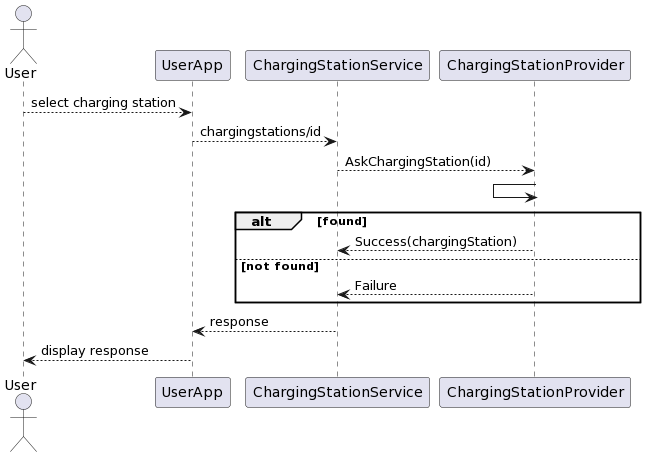
\includegraphics[width=\textwidth]{images/ask-station.png}
    \caption{Diagramma delle sequenze per la visualizzazione dello stato di una stazione di ricarica}
    \label{fig:ask-station}
\end{figure}

\paragraph{Visualizzazione dello stato di tutte le stazioni di ricarica all'interno della mappa}
L'utente interagisce con l'applicazione utente ("UserApp") e seleziona la visualizzazione della mappa.

L'applicazione utente invia quindi una richiesta per ottenere l'elenco di tutte le stazioni di ricarica disponibili al Charging Station Service. Il Servizio a sua volta comunica con il Provider.

Esso cerca tutte le stazioni di ricarica disponibili all'interno del suo registro. Successivamente, restituisce l'elenco completo delle stazioni di ricarica al Charging Station Service.

Quest'ultimo, a sua volta, restituisce l'elenco delle stazioni di ricarica all'applicazione utente. Infine, quest'ultima mostra le stazioni di ricarica all'interno della mappa all'utente.

Questa interazione è riassunta nel seguente diagramma di sequenza:

\begin{figure}[htbp]
    \centering
    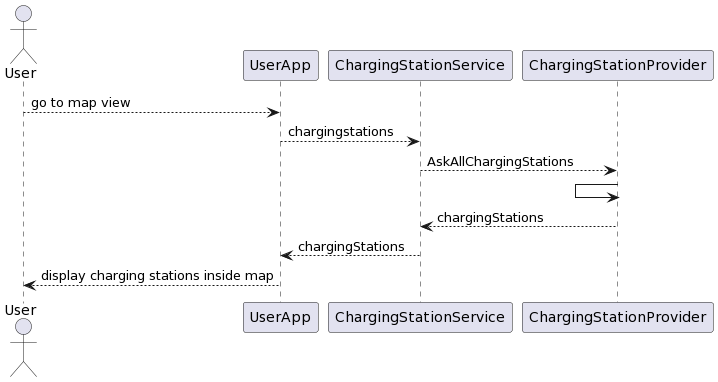
\includegraphics[width=\textwidth]{images/ask-all-stations.png}
    \caption{Diagramma delle sequenze per la visualizzazione dello stato di tutte le stazioni di ricarica all'interno della mappa}
    \label{fig:ask-all-stations}
\end{figure}

\paragraph{Prenotazione di una stazione di ricarica}
L'utente interagisce con l'applicazione utente e seleziona una stazione di ricarica da prenotare.

Successivamente, l'utente invia una richiesta di prenotazione al Charging Station Service tramite l'applicazione utente. Il Service comunica con il Charging Station Provider per richiedere la prenotazione della stazione selezionata.

Il Provider, a sua volta, comunica con il Charging Station Actor per effettuare la prenotazione. Se la stazione di ricarica è stata trovata, il Provider richiede all'attore della Stazione di Ricarica la prenotazione, il quale gli comunica l'esito.

Nel caso in cui la stazione di ricarica sia libera, l'attore della Stazione di Ricarica conferma la prenotazione e comunica al Provider che la prenotazione è avvenuta con successo. Il Provider, a sua volta, comunica al Service il successo della prenotazione, il quale comunica l'esito positivo all'applicazione utente.

Tuttavia, se la stazione di ricarica è già prenotata o è attualmente in uso per la ricarica, l'attore della Stazione di Ricarica comunica al Provider che la prenotazione non può essere effettuata. Il Provider comunica quindi al Service il fallimento della prenotazione, e questo a sua volta comunica all'applicazione utente l'esito negativo della prenotazione.

Nel caso in cui la stazione di ricarica non venga trovata, il Provider lo comunica al Service, che comunica quindi all'applicazione utente che la stazione di ricarica selezionata non è disponibile.\\

Questa interazione è riassunta nel seguente diagramma di sequenza:

\begin{figure}[htbp]
    \centering
    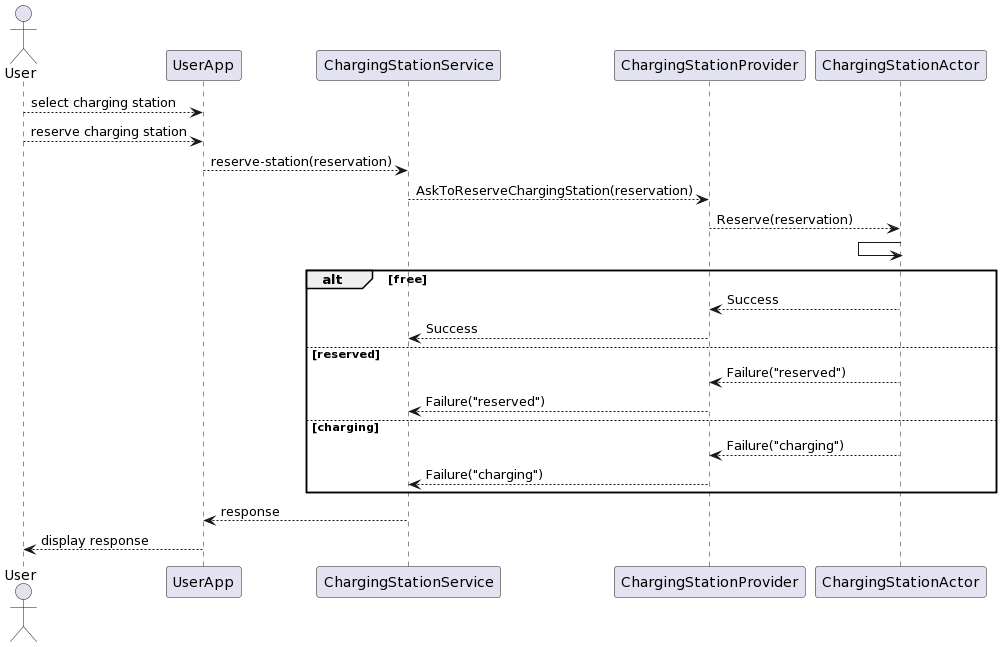
\includegraphics[width=\textwidth]{images/reserve-station.png}
    \caption{Diagramma delle sequenze per la prenotazione di una stazione di ricarica}
    \label{fig:reserve-station}
\end{figure}

\paragraph{Richiesta di ricarica di un veicolo}
L'utente interagisce con l'applicazione utente  e seleziona una stazione di ricarica. Successivamente, l'utente legge un codice QR associato alla stazione.

L'applicazione utente richiede quindi la possibilità di effettuare una ricarica presso la stazione selezionata e comunica al Charging Station Service la richiesta di ricarica. Il Servizio Stazioni di Ricarica comunica con il Charging Station Provider per richiedere l'autorizzazione alla ricarica.

Il Provider, a sua volta, comunica con il Charging Station Actor per autorizzare la ricarica.

Nel caso in cui la stazione di ricarica sia libera, l'attore comunica al Provider il successo della richiesta. Questo, a sua volta, comunica al Service il successo dell'autorizzazione, che lo comunica all'applicazione utente.

Se la stazione di ricarica è già prenotata, l'attore della Stazione di Ricarica verifica la prenotazione o lo stato di carica attuale. Se la prenotazione è valida, l'attore autorizza la ricarica. Altrimenti, se la prenotazione non è valida, l'attore comunica che la stazione non può essere utilizzata per la ricarica. Il Provider comunica quindi al Service il fallimento dell'autorizzazione, e questo a sua volta comunica all'applicazione utente l'esito negativo della richiesta di ricarica.

Se la stazione di ricarica è attualmente in uso, l'attore comunica che la stazione non può essere utilizzata per la ricarica. Il Provider comunica quindi al Service il fallimento dell'autorizzazione, e questo a sua volta comunica all'applicazione utente l'esito negativo della richiesta di ricarica.

Nel caso in cui la stazione di ricarica non venga trovata (caso "not found"), il Fornitore Stazioni di Ricarica comunica al Servizio Stazioni di Ricarica che la stazione non è stata trovata. Il Servizio Stazioni di Ricarica comunica quindi all'applicazione utente che la stazione di ricarica selezionata non è disponibile.

Questa interazione è riassunta nel seguente diagramma di sequenza:

\begin{figure}[!htbp]
    \centering
    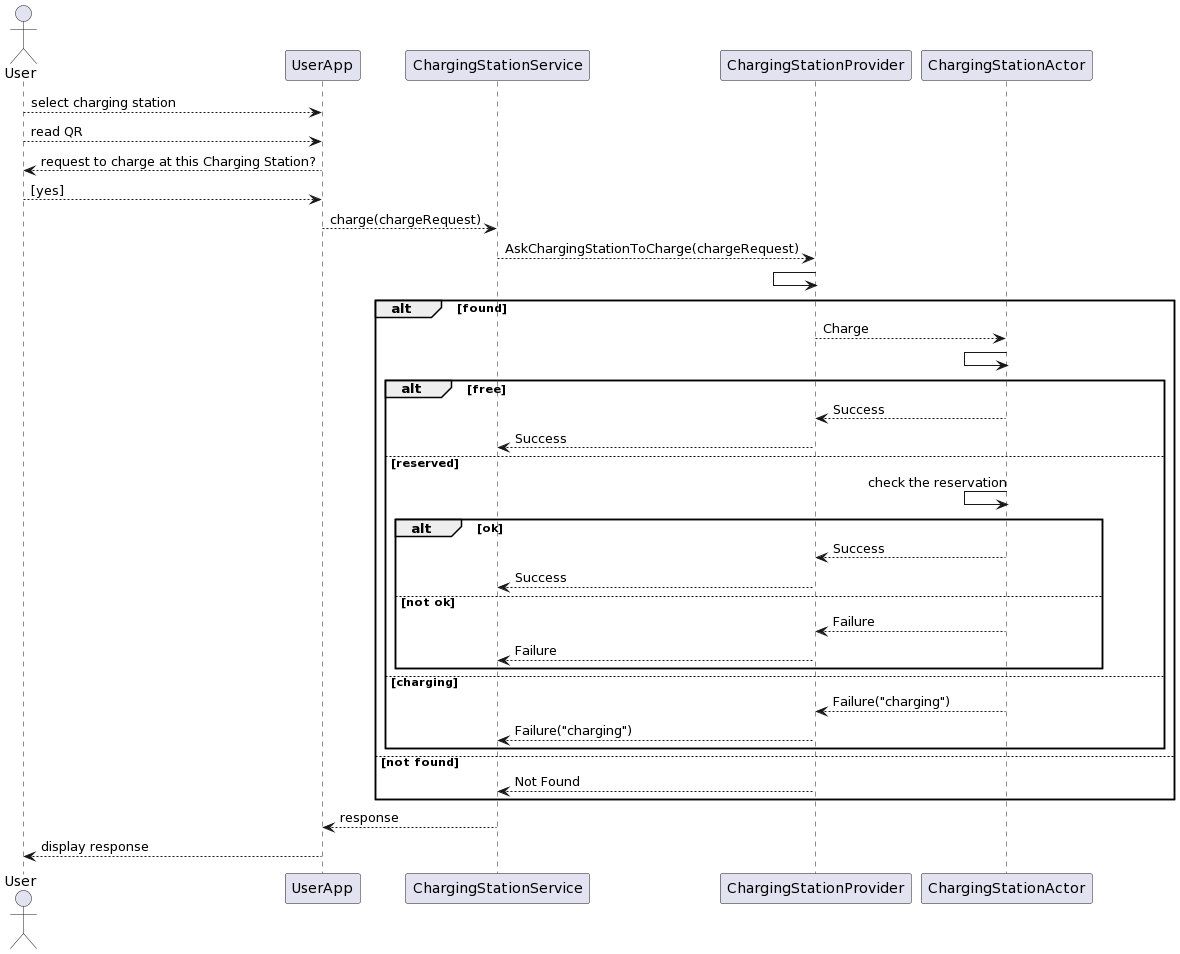
\includegraphics[width=\textwidth]{images/charge.png}
    \caption{Diagramma delle sequenze per la richiesta di ricarica di un veicolo}
    \label{fig:charge}
\end{figure}
\clearpage

\subsection{Design di Dettaglio}
%TODO: spiega le interazioni tra gli attori e componenti del sistema, con descrizione sia testuale che con diagrammi di sequenza.
La fase di Design di Dettaglio affronta la progettazione del sistema ad un livello di granularità più fine, siccome è in questa fase che ci si occupa di progettare i singoli componenti del sistema ed il loro protocollo di interazione.\\

\subsubsection{User Domain}
%TODO: spiegare le scelte di design principali della user app e dell'auth server con eventuali schemi

L'applicazione web lato client si occupa di fornire all'utente le informazioni raccolte dal server
e gestire l'ottenimento di dati da sensori quali GPS e fotocamera.\\

Per prima cosa, l'applicazione fornisce all'utente le funzionalità di registrazione e login,
che concederà all'utente una migliore esperienza di utilizzo, dando anche la possibilità di
memorizzare le colonnine di interesse, salvate all'interno del database.\\

Successivamente al login, l'utente verrà indirizzato sulla sua home page, dalla quale avrà la possibilità
di visionare le proprie colonnine d'interesse, un link diretto alla mappa delle colonnine ed uno
alla scansione del codice QR. Se presenti, dalle colonnine d'interesse sarà possibile accedere
direttamente alla pagina di prenotazione della colonnina.\\

La mappa delle colonnine è una pagina che mostra all'utente la posizione di tutte le colonnine ed il loro stato attuale,
nel momento in cui accede alla pagina, gli verrà chiesto di utilizzare la propria posizione,
se acconsente vedrà la sua posizione sulla mappa e le colonnine più vicine ad essa.\\

La scansione del codice QR permette all'utente di accedere alla pagina di caricamento presso la colonnina,
questo è l'unico modo in cui la colonnina può cambiare il suo stato in "caricamento", siccome si suppone che
presso ogni colonnina sia fisicamente presente un codice QR che la identifica univocamente.\\

Nel momento in cui l'utente fa una richiesta di prenotazione o caricamento, verrà contattato il server Akka,
che in base allo stato e disponibilità della colonnina, risponderà di conseguenza all'utente.\\

Sono state definite chiaramente le interfacce di comunicazione tra i vari componenti dell'User Domain,
assicurando una fluida trasmissione dei dati e dei messaggi tra l'app, l'auth server, il server akka ed il database.
Questo approccio dettagliato alla progettazione ha permesso di garantire un'interazione sicura e
affidabile tra gli utenti e il sistema.\\

Nel complesso, il design di dettaglio dell'User Domain è stato realizzato con l'obiettivo di offrire
un'interfaccia utente intuitiva e una gestione dell'autenticazione robusta, garantendo al contempo
la sicurezza e l'efficienza del sistema nel suo complesso.

\subsubsection{Charging Station Domain}
Per quanto riguarda il dominio delle Charging Station, il gruppo ha deciso di utilizzare il paradigma ad \textbf{attori} per modellare il comportamento dei componenti del dominio e la
metodologia di interazione tra essi. \\

In questo paradigma, un attore è un'entità computazionale che può ricevere messaggi, elaborarli e rispondere con altri messaggi. Gli attori sono organizzati in gerarchie, dove ogni attore ha un solo attore padre e può avere più attori figli.\\
Ogni attore possiede una \textbf{mailbox}, ovvero una coda di messaggi in entrata, e un \textbf{behavior}, ovvero un insieme di regole che definiscono il comportamento dell'attore alla ricezione di un messaggio.\\

Una particolarità del modello ad attori è che può efficacemente modellare una macchina a stati finiti, in quanto l'attore può cambiare il suo comportamento in base al messaggio ricevuto e gli stati finiti corrispondono al set di messaggi ai quali l'attore può rispondere.\\
Questo ha permesso di modellare efficacemente il comportamento delle Charging Station, che possono trovarsi in uno dei seguenti stati:
\begin{itemize}
    \item \textbf{Free}: la stazione è disponibile per la ricarica.
    \item \textbf{Reserved}: la stazione è stata prenotata.
    \item \textbf{Charging}: la stazione è attualmente in uso per la ricarica.
\end{itemize}

La macchina a stati finiti per il Charging Station Actor è riassunta nel seguente diagramma:

\begin{figure}[htbp]
    \centering
    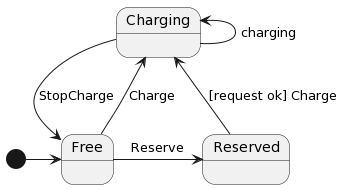
\includegraphics[width=\textwidth]{images/cs-state.png}
    \caption{Diagramma della macchina a stati finiti per il Charging Station Actor}
    \label{fig:cs-state}
\end{figure}


%Devono essere esposte le scelte progettuali operate nelle varie fasi di sviluppo dell'elaborato.\\

%In questa sezione devono essere documentati gli schemi di progetto relativamente all'architettura complessiva del sistema e alle sue componenti di rilievo che possano meritare un'analisi di dettaglio. Per le componenti software si può ricorrere ad esempio a diagrammi delle classi, di sequenza, stato, attività. Per le componenti hardware è possibile includere opportuni schemi in grado di descrivere l'architettura fisica adottata.\\

%Vincoli circa la lunghezza della sezione (escluse didascalie, tabelle, testo nelle immagini, schemi):

%\vspace{1cm}
%\begin{tabular}{l|rr}
% & Numero minimo di battute & Numero massimo di battute \\
% \hline
% 1 componente & 9000 & 18000 \\
% 2 componenti & 12000 & 21000 \\
% 3 componenti & 15000 & 24000 \\
% \hline
%\end{tabular}


\newpage

%----------------------------------------------------------------------------------------
%	IMPLEMENTAZIONE
%----------------------------------------------------------------------------------------

\section{Implementazione}\label{sec:implementazione}


\subsection{User Domain}

Per quanto riguarda l'implementazione dell'applicazione con cui si interfaccia l'utente, è stato deciso di utilizzare il framework Svelte. Questa scelta è stata dettata da un'approfondita analisi delle opzioni disponibili e da diverse considerazioni chiave che hanno guidato questa decisione.

\subsubsection{Svelte: Leggerezza e Performance}

Svelte è emerso come la scelta ideale per l'implementazione dell'interfaccia utente. La sua caratteristica distintiva è la mancanza di un Virtual DOM, a differenza di framework concorrenti come React o Vue. Invece, Svelte utilizza un compilatore che traduce il codice scritto in JavaScript, HTML e CSS direttamente in codice JavaScript nativo altamente ottimizzato. Questo si traduce in un'applicazione con un codice molto più leggero e una maggiore velocità rispetto ad altri framework. La leggerezza è essenziale per garantire un'esperienza utente fluida, soprattutto su dispositivi con risorse limitate.

\subsubsection{Semplicità e Velocità di Sviluppo}

Oltre alla performance, Svelte offre una curva di apprendimento molto meno ripida rispetto ad altri framework. La sua sintassi dichiarativa e la facilità con cui è possibile definire componenti rendono la scrittura del codice più efficiente. Un aspetto chiave è il sistema di "store" di Svelte. Nel codice fornito, notiamo l'uso dei moduli `writable` e `createEventDispatcher` per creare e gestire uno store denominato "Stations". Questo store è fondamentale per la gestione dello stato delle stazioni di ricarica all'interno dell'applicazione. Le funzioni come `fetchStations`, `charge`, `reserve`, `addFavourite`, e `removeFavourite` operano su questo store per mantenere una visione coerente e reattiva dei dati in tutta l'applicazione.

\subsubsection{Integrazione con Altre Tecnologie}

L'integrazione è stata un altro punto cruciale nella scelta di Svelte. Ad esempio, l'applicazione utilizza Leaflet, una libreria JavaScript per la creazione di mappe interattive. L'integrazione di Leaflet con Svelte è stata fluida, consentendo la visualizzazione delle stazioni di ricarica sulla mappa in modo efficace ed efficiente. Inoltre, l'applicazione è scritta in TypeScript, un linguaggio che aggiunge tipizzazione statica a JavaScript. Questo migliora la manutenibilità del codice e aiuta a prevenire errori comuni durante lo sviluppo.

\subsection{Auth Server}

Tra le funzionalità dell'applicazione, troviamo la possibilità di effettuare la registrazione personale ed il login. Per gestire queste funzionalità è stato utilizzato il framework Express.js, che offre una solida base per la creazione di un server web in Node.js. Le motivazioni dietro questa scelta sono state ponderate attentamente.

\subsubsection{Express.js: Facilità d'Uso e Configurabilità}

Express.js è noto per la sua facilità d'uso nella creazione di server web. La sua flessibilità lo rende una scelta eccellente per gestire le route, le richieste HTTP e le risposte nell'applicazione. Inoltre, è stato configurato per gestire le opzioni CORS (Cross-Origin Resource Sharing), il che consente di consentire o limitare l'accesso ai servizi del server da parte di domini esterni. Questo è fondamentale per garantire una comunicazione sicura tra il frontend e il backend.

\subsubsection{Memorizzazione dei Dati Utente con MongoDB}

Per memorizzare i dati degli utenti, è stata fatta una scelta significativa nell'adozione di MongoDB, un database non relazionale orientato ai documenti. Questa decisione è stata guidata da diverse considerazioni fondamentali.

\subsubsection{Flessibilità Strutturale}

Innanzitutto, MongoDB offre una flessibilità strutturale significativa. Ciò significa che è possibile gestire dati eterogenei senza la necessità di un rigoroso schema fisso. Questo si è rivelato particolarmente utile durante lo sviluppo, consentendo di adattarsi facilmente alle esigenze cambianti dell'applicazione.

\subsubsection{Scalabilità Orizzontale}

In secondo luogo, MongoDB è noto per la sua scalabilità orizzontale. Questa caratteristica è cruciale quando si gestiscono grandi volumi di dati e carichi di traffico in crescita. L'architettura di MongoDB consente di aggiungere nuovi nodi al cluster in modo relativamente semplice, consentendo all'applicazione di crescere in modo fluido con il suo successo.

\subsubsection{Velocità di Sviluppo e Integrazione con JavaScript}

Infine, MongoDB si è dimostrato un'ottima scelta per accelerare lo sviluppo. La sua capacità di memorizzare e recuperare dati in un formato JSON-like si integra perfettamente con il mondo JavaScript, garantendo coerenza tra il modello dati del backend e quello del frontend.


\subsection{Charging Station Domain}
Per quanto riguarda l'implementazione delle componenti del Charging Station Domain, vista la scelta fatta di progettare i sotto-componenti del dominio attraverso il modello ad attori, la scelta su come implementarli è
ricaduta sul framework Akka. Akka è un toolkit open-source per la creazione di applicazioni concorrenti e distribuite basate sul modello ad attori. Il framework è scritto in Scala, ma è possibile utilizzarlo anche con Java, tuttavia in questa sede
si è preferito utilizzare il linguaggio Scala poichè più flessibile, conciso e potente della controparte Java, oltre al fatto che offre un'esperienza di sviluppo migliore col framework Akka.\\
In particolare, è stata scelta l'api \textbf{Akka Typed}, che permette di definire gli attori attraverso un sistema di tipi, rendendo più semplice la gestione degli stessi.\\

Gli attori implementati in Akka sono stati i seguenti:
\begin{itemize}
      \item Charging Station Actor
      \item Charging Station Provider
      \item Charging Station Service
\end{itemize}

Per ognuno di essi, l'implementazione ha seguito il seguente schema:\\

\paragraph{Definizione dei messaggi scambiati tra gli attori:}
in Akka Typed, l'attore è rappresentato dal concetto di \textbf{Behavior<T>}, che è un'astrazione che rappresenta il ciclo di vita di un attore. In particolare, un Behavior è un'interfaccia funzionale che prende in input un messaggio di tipo T e restituisce un nuovo Behavior.\\
Il primo passo è stato dunque quello di definire i messaggi scambiati tra gli attori, ovvero i tipi T.\\
Per prima cosa, per ogni attore è stato definito un sealed trait base \textbf{Request} da estendere per ogni diverso messaggio che l'attore può ricevere.\\
Dopodichè, con l'aiuto degli schemi fatti in fase di progettazione, sono state create, per ogni attore, diverse case classes le quali estendono Request e rappresentano i diversi messaggi specifici che l'attore può ricevere.\\
Segue un esempio di definizione dei messaggi per l'attore Charging Station Actor:
\begin{lstlisting}[language=scala]
object ChargingStationEvents:
      sealed trait Request
      case class AskState(replyTo: ActorRef[ChargingStationProvider.Request]) extends Request
      case class Charge(request: ChargeRequest, replyTo: ActorRef[ChargeRequestResult]) extends Request
      case class Reserve(reservation: Reservation, replyTo: ActorRef[ReservationResult]) extends Request
      case class StopCharge() extends Request
\end{lstlisting}

\paragraph{Definizione delle reazioni ai messaggi:}
Come anticipato, il Behavior<T> è un'interfaccia funzionale che prende in input un messaggio di tipo T e restituisce un nuovo Behavior.\\
Dunque, per completare l'implementazione di un attore è necessario fornire un implementazione coerente di Behavior<T>. A tale scopo, Akka fornisce svariate funzioni di factory racchiuse nell'object \textbf{Behaviors}, che permettono di creare Behavior<T> in modo semplice e conciso.\\
A seconda della complessità dell'attore da implementare, sono state utilizzate le seguenti funzioni di factory:
\begin{itemize}
      \item \textbf{Behaviors.receive:} questa funzione permette di creare un Behavior<T> che reagisce a un messaggio di tipo T. In particolare, prende in input una funzione che prende in input il messaggio di tipo T e l'\textbf{Actor Context} e restituisce un Behavior<T>.\\
            L'Actor Context è un elemento chiave del framework Akka, poichè permette all'attore di manipolare od ottenere informazioni circa il suo contesto di esecuzione. Questo oggetto è necessario laddove un attore debba spawnare un attore figlio, accedere al proprio riferimento univoco, o utilizzare funzionalità di logging.\\
            Questa factory è stata utilizzata per implementare Charging Station Actor e Charging Station Provider.
      \item \textbf{Behaviors.receiveMessage:} questa funzione permette di creare un Behavior<T> che reagisce a un messaggio di tipo T. In particolare, prende in input una funzione che prende in input il messaggio di tipo T e restituisce un Behavior<T>.\\
            È una versione più concisa della receive classica poichè non necessita dell'Actor Context. Questa factory è stata utilizzata per implementare Charging Station Service.
      \item \textbf{Behaviors.setup:} questa funzione non reagisce a nessun messaggio, ma permette di eseguire del codice una volta che l'attore è stato spawnato. In particolare, prende in input una funzione che prende in input l'Actor Context e restituisce un Behavior<T>.\\
            Questa factory è stata utilizzata per implementare Charging Station Actor e Charging Station Provider.	
\end{itemize}

Di seguito un esempio semplificato di implementazione di un attore utilizzando Behaviors.setup e Behaviors.receive:\\

\begin{lstlisting}[language=scala]
object ChargingStationProvider:
      def apply(): Behavior[ChargingStationProvider.Request] = 
            Behaviors setup { context =>
                  // esegui operazioni preliminari dipendenti dall'Actor Context
                  running() // separiamo il codice del setup da eseguire una sola volta con il codice effettivo del Behavior
            }
      private def running(): Behavior[ChargingStationProvider.Request] = 
            Behaviors receive { (context, message) =>
                  // reagisci al messaggio
                  running() // ritorna ricorsivamente questo Behavior
            }
\end{lstlisting}

\subsubsection{Creazione di un cluster di attori}

\subsubsection*{Serializzazione intra cluster}

\subsubsection*{Marshalling e Unmarshalling}

\subsection{Tecnologie impiegate}

In questa sezione, verranno presentate in dettaglio le principali tecnologie utilizzate per implementare il sistema e le motivazioni che ci hanno spinto a sceglierle.

\subsubsection{Applicazione utente}

Per l'implementazione dell'applicazione utente, sono state impiegate diverse tecnologie chiave:

\begin{itemize}
      \item \textbf{Svelte:} Svelte è il framework front-end principale utilizzato per la creazione dell'interfaccia utente dell'applicazione. La sua caratteristica distintiva è la compilazione del codice Svelte in JavaScript altamente ottimizzato. Questo framework permette di scrivere codice dichiarativo che si traduce in un'applicazione web reattiva ed efficiente.

      \item \textbf{Svelte Kit:} Svelte Kit è una libreria aggiuntiva che semplifica la gestione delle route e delle pagine in un'applicazione Svelte. Questo è fondamentale per creare un'applicazione a pagine multiple in modo strutturato e organizzato.

      \item \textbf{Leaflet:} Leaflet è una libreria JavaScript utilizzata per creare mappe interattive. È stata impiegata nell'applicazione per l'integrazione delle mappe e la visualizzazione delle stazioni di ricarica per veicoli elettrici.

      \item \textbf{TypeScript:} TypeScript è un linguaggio di programmazione che aggiunge tipizzazione statica a JavaScript. Questo miglioramento della tipizzazione rende il codice più affidabile e agevola la manutenzione.

      \item \textbf{Vite:} Vite è un bundler e un task runner veloce progettato per lo sviluppo front-end. Grazie al suo sistema di moduli nativo e alla ricarica a caldo, semplifica notevolmente lo sviluppo e l'ottimizzazione del codice.

      \item \textbf{Svelte Geolocation:} La dipendenza "svelte-geolocation" è stata utilizzata per accedere alla funzionalità di geolocalizzazione del dispositivo all'interno dell'applicazione. Questo è utile per determinare la posizione dell'utente e fornire informazioni basate sulla sua posizione, ad esempio la visualizzazione delle stazioni di ricarica più vicine.

      \item \textbf{Svelte QR Scanner:} "Svelte-qr-scanner" è stato integrato nell'applicazione per consentire la scansione dei codici QR. Questa funzionalità è utilizzata per diverse finalità, ad esempio la lettura di QR code per lo sblocco di una colonnina ed il conseguente inizio della ricarica.
\end{itemize}

\subsubsection{Authentication server}

Per quanto riguarda il server utilizzato per l'autenticazione, sono state utilizzate le seguenti tecnologie:

\begin{itemize}
      \item \textbf{Express.js:} Express è un framework web per Node.js che semplifica la creazione di server web. È utilizzato per gestire le route, le richieste HTTP e le risposte nell'applicazione.

      \item \textbf{MongoDB:} MongoDB è un database non relazionale orientato ai documenti. È utilizzato per memorizzare i dati dell'applicazione in formato JSON-like. La scelta di MongoDB è stata motivata dalla flessibilità strutturale, dalla scalabilità orizzontale e dalla facilità di sviluppo.

      \item \textbf{Mongoose:} Mongoose è una libreria Node.js che semplifica l'interazione con il database MongoDB. È utilizzato per definire gli schemi dei dati e per eseguire operazioni di query nel database in modo più intuitivo.

      \item \textbf{bcrypt:} bcrypt è una libreria per la crittografia delle password. È utilizzata per proteggere le password degli utenti nel database, garantendo che siano memorizzate in modo sicuro.

      \item \textbf{CORS:} CORS (Cross-Origin Resource Sharing) è una tecnologia che consente di gestire le richieste HTTP provenienti da origini diverse. È utilizzata per consentire o limitare l'accesso ai servizi del server da parte di domini esterni.

      \item \textbf{dotenv:} dotenv è un modulo che permette di caricare variabili d'ambiente da un file di configurazione. È utilizzato per gestire le variabili d'ambiente nell'applicazione, consentendo la configurazione di parametri sensibili come le chiavi segrete.

      \item \textbf{jsonwebtoken:} jsonwebtoken è una libreria per la gestione dei JSON Web Token (JWT). È utilizzata per l'autenticazione e l'autorizzazione degli utenti nell'applicazione.
\end{itemize}

\paragraph{Perchè MongoDB}

Le scelte che hanno portato alla decisione dell'utilizzo di MongoDB anzichè
di un database relazionale sono state le seguenti:

\begin{itemize}
      \item \textbf{Flessibilità nella struttura dei dati:} MongoDB consente di gestire

            dati eterogenei senza la necessità di uno schema fisso.

      \item \textbf{Scalabilità orizzontale:} La capacità di scalare orizzontalmente è
            cruciale per gestire grandi volumi di dati e carichi di traffico crescenti.

      \item \textbf{Velocità di sviluppo:} MongoDB semplifica lo sviluppo rapido,
            consentendo di memorizzare e recuperare dati in formato JSON-like.

      \item \textbf{Integrazione nativa con JavaScript:} Si integra bene con applicazioni
            JavaScript, fornendo coerenza tra il modello dati del backend e quello del frontend.
\end{itemize}

\subsubsection{Akka HTTP}



% \subsection{User App - A}

% %Considerazioni generali sulle particolarità di svelte

% Per quanto riguarda l'implementazione dell'applicazione con cui si interfaccia l'utente,
% è stato deciso di utilizzare il framework Svelte. Questa scelta è stata dettata dal fatto
% che Svelte è un framework molto leggero, che non utilizza un Virtual DOM, ma che si basa
% su un compilatore che traduce il codice scritto in Javascript, HTML e CSS in codice Javascript
% nativo. Questo permette di avere un codice molto più leggero e veloce rispetto ad altri
% framework come React o Vue. Inoltre, Svelte è molto semplice da utilizzare e permette
% di creare applicazioni web in modo molto intuitivo e veloce.


% \subsubsection{Svelte store}
% Lo "store" in Svelte è un meccanismo per gestire lo stato dell'applicazione in modo reattivo e condiviso tra le diverse parti dell'applicazione. Nella porzione di codice fornita, vengono utilizzati i moduli \texttt{writable} e \texttt{createEventDispatcher} per creare e gestire uno store denominato "Stations". Ecco una breve descrizione di ciò che viene fatto nel codice:
% \begin{enumerate}[label=\arabic*.]
%       \item \textbf{Creazione dello Store "Stations"}: La riga
%             \texttt{export const Stations = writable([])} inizializza uno store
%             Svelte chiamato "Stations" utilizzando la funzione \texttt{writable}.
%             Questo store sarà utilizzato per memorizzare e condividere un elenco
%             di stazioni di ricarica all'interno dell'applicazione.

%       \item \textbf{Definizione di Funzioni per Interagire con lo Store}:
%             \begin{enumerate}[label=\arabic{enumi}.\arabic*]
%                   \item \textit{fetchStations}: Questa funzione effettua una richiesta
%                         HTTP per recuperare l'elenco delle stazioni di ricarica dal server (AKKA SERVER)
%                         e poi lo trasforma in un formato appropriato. Infine, aggiorna il valore dello
%                         store "Stations" utilizzando \textit{Stations.set(newStations)}. In questo modo,
%                         l'elenco delle stazioni è disponibile globalmente all'interno dell'applicazione.

%                   \item \texttt{charge}: Questa funzione invia una richiesta HTTP al server AKKA per avviare una sessione di ricarica per un utente presso una stazione di ricarica specifica. Se l'operazione ha successo, l'applicazione viene reindirizzata alla pagina principale.

%                   \item \texttt{reserve}: Simile a \texttt{charge}, questa funzione invia una richiesta HTTP per prenotare una stazione di ricarica e reindirizza l'applicazione alla pagina principale se ha successo.
%                   \item \textit{addFavourite}: Questa funzione invia una
%                         richiesta HTTP al server (EXPRESS SERVER) per aggiungere una stazione
%                         di ricarica ai preferiti di un utente. Se la richiesta ha successo, viene
%                         generato un evento personalizzato per notificare altre parti dell'applicazione.

%                   \item \texttt{removeFavourite}: Simile a \texttt{addFavourite}, questa funzione invia una richiesta HTTP per rimuovere una stazione dai preferiti di un utente e genera un evento se l'operazione ha successo.
%             \end{enumerate}
% \end{enumerate}


% \subsection{Auth Server}

% % parlare di express e nodejs e mongodb

% Tra le funzionalità dell'applicazione, troviamo la possibilità di effettuare la
% registrazione personale ed il login. Per gestire queste funzionalità è stato utilizzato
% il framework Express.js, che permette di creare un server web in Node.js e include
% la configurazione delle opzioni CORS per consentire richieste da qualsiasi origine.
% Inoltre, per memorizzare i dati degli utenti, è stato utilizzato MongoDB,
% un database non relazionale che permette di memorizzare i dati in formato JSON.
% Per interfacciarsi con il database, è stato utilizzato il modulo Mongoose, che
% permette di definire degli schemi per i dati che vengono memorizzati nel database.


% \subsection{Tecnologie impiegate - A}

% In questa sezione verranno presentate le principali tecnologie utilizzate per implementare il sistema e le motivazioni che ci hanno spinto a sceglierle.

% \subsubsection{Applicazione utente}
% Le tecnologie principali utilizzate per l'implementazione dell'applicazione utente sono:

% \begin{itemize}
%       \item \textbf{Svelte:} Svelte è il framework front-end principale utilizzato per la creazione
%             dell'interfaccia utente dell'applicazione. La sua caratteristica distintiva è la compilazione
%             del codice Svelte in JavaScript altamente ottimizzato. Questo framework permette di scrivere
%             codice dichiarativo che si traduce in un'applicazione web reattiva ed efficiente.

%       \item \textbf{Svelte Kit:} Svelte Kit è una libreria aggiuntiva che semplifica la gestione
%             delle route e delle pagine in un'applicazione Svelte. Questo è fondamentale per creare
%             un'applicazione a pagine multiple in modo strutturato e organizzato.

%       \item \textbf{Leaflet:} Leaflet è una libreria JavaScript utilizzata per creare mappe
%             interattive. È stata impiegata nell'applicazione per l'integrazione delle mappe e la
%             visualizzazione delle stazioni di ricarica per veicoli elettrici.

%       \item \textbf{TypeScript:} TypeScript è un linguaggio di programmazione che aggiunge
%             tipizzazione statica a JavaScript. Questo miglioramento della tipizzazione rende
%             il codice più affidabile e agevola la manutenzione.

%       \item \textbf{Vite:} Vite è un bundler e un task runner veloce progettato per lo
%             sviluppo front-end. Grazie al suo sistema di moduli nativo e alla ricarica a caldo,
%             semplifica notevolmente lo sviluppo e l'ottimizzazione del codice.

%       \item \textbf{Svelte Geolocation:} La dipendenza "svelte-geolocation" è stata utilizzata
%             per accedere alla funzionalità di geolocalizzazione del dispositivo all'interno
%             dell'applicazione. Questo è utile per determinare la posizione dell'utente e fornire
%             informazioni basate sulla sua posizione, ad esempio la visualizzazione delle stazioni di ricarica
%             più vicine.

%       \item \textbf{Svelte QR Scanner:} "Svelte-qr-scanner" è stato integrato nell'applicazione
%             per consentire la scansione dei codici QR. Questa funzionalità è utilizzata per diverse
%             finalità, ad esempio la lettura di QR code per lo sblocco di una colonnina ed il
%             conseguente inizio della ricarica.
% \end{itemize}

% \subsubsection{Authentication server}

% Per quanto riguarda il server utilizzato per l'autenticazione sono state utilizzate le seguenti tecnologie:

% \begin{itemize}

%       \item \textbf{express:} Express è un framework web per Node.js che semplifica
%             la creazione di server web. È utilizzato per gestire le route, le richieste
%             HTTP e le risposte nell'applicazione.

%       \item \textbf{mongodb:} MongoDB è un database non relazionale orientato ai
%             documenti. È utilizzato per memorizzare i dati dell'applicazione in formato
%             JSON-like. MongoDB è una scelta comune per applicazioni che richiedono scalabilità
%             e flessibilità nella gestione dei dati.

%       \item \textbf{mongoose:} Mongoose è una libreria Node.js che semplifica l'interazione
%             con il database MongoDB. È utilizzato per definire gli schemi dei dati e per
%             eseguire operazioni di query nel database in modo più intuitivo.

%       \item \textbf{bcrypt:} bcrypt è una libreria per la crittografia delle password.
%             È utilizzata per proteggere le password degli utenti nel database, garantendo che
%             siano memorizzate in modo sicuro.

%       \item \textbf{cors:} CORS (Cross-Origin Resource Sharing) è una tecnologia che
%             consente di gestire le richieste HTTP provenienti da origini diverse. È utilizzata
%             per consentire o limitare l'accesso ai servizi del server da parte di domini esterni.

%       \item \textbf{dotenv:} dotenv è un modulo che permette di caricare variabili
%             d'ambiente da un file di configurazione. È utilizzato per gestire le variabili
%             d'ambiente nell'applicazione, consentendo la configurazione di parametri
%             sensibili come le chiavi segrete.

%       \item \textbf{jsonwebtoken:} jsonwebtoken è una libreria per la gestione dei
%             JSON Web Token (JWT). È utilizzata per l'autenticazione e l'autorizzazione
%             degli utenti nell'applicazione.

% \end{itemize}

% Le scelte che hanno portato alla decisione dell'utilizzo di MongoDB anzichè
% di un database relazionale sono state le seguenti:

% \begin{itemize}
%       \item \textbf{Flessibilità nella struttura dei dati:} MongoDB consente di gestire

%             dati eterogenei senza la necessità di uno schema fisso.

%       \item \textbf{Scalabilità orizzontale:} La capacità di scalare orizzontalmente è
%             cruciale per gestire grandi volumi di dati e carichi di traffico crescenti.

%       \item \textbf{Velocità di sviluppo:} MongoDB semplifica lo sviluppo rapido,
%             consentendo di memorizzare e recuperare dati in formato JSON-like.

%       \item \textbf{Integrazione nativa con JavaScript:} Si integra bene con applicazioni
%             JavaScript, fornendo coerenza tra il modello dati del backend e quello del frontend.
% \end{itemize}



%Esporre i principali problemi affrontati durante l'effettiva realizzazione delle componenti hardware/software e illustrare le soluzioni implementative adottate. Se l'elaborato ha previsto l'utilizzo di tecnologie già disponibili sul mercato, discuterne brevemente le caratteristiche e motivarne l'adozione rispetto ad altre soluzioni assimilabili.\\

%\textbf{NOTA: in questa sezione devono essere riportate esclusivamente le porzioni di codice ritenute particolarmente significative. Il codice sorgente nella sua interezza, opportunamente commentato, deve essere consegnato separatamente dalla relazione in un archivio compresso.}\\


%Vincoli circa la lunghezza della sezione (escluse didascalie, tabelle, testo nelle immagini, schemi):

%\vspace{1cm}
%\begin{tabular}{l|rr}
%                 & Numero minimo di battute & Numero massimo di battute \\
%    \hline
%    1 componente & 5000                     & 11000                     \\
%    2 componenti & 8000                     & 16000                     \\
%    3 componenti & 10000                    & 21000                     \\
%    \hline
%\end{tabular}


\newpage
%----------------------------------------------------------------------------------------
%	TESTING E PERFORMANCE
%----------------------------------------------------------------------------------------

\section{Testing e performance}
%intro + scalatest + server express w/postman

Il testing è un processo fondamentale nello sviluppo del software che mira a verificare se un'applicazione
funziona correttamente e soddisfa i requisiti specificati. Serve a individuare e correggere eventuali
errori o difetti nel codice, garantendo che il software sia affidabile, stabile e conforme alle aspettative degli utenti.

L'importanza di testing e performance engineering risiede nella garanzia della qualità del software.
Il testing assicura che il software sia privo di bug e funzioni correttamente, migliorando la fiducia
degli utenti e riducendo i costi legati a eventuali correzioni post-lancio. Le prestazioni,
d'altra parte, influenzano direttamente l'esperienza utente e la soddisfazione del cliente.
Un'applicazione lenta o instabile può respingere gli utenti.

\subsection{Scalatest}
ScalaTest è un framework di testing per il linguaggio di programmazione Scala.
È stato progettato per consentire una varietà di stili di testing, tra cui il testing unitario,
il testing di integrazione e il testing di accettazione.\\

All'interno del progetto, ScalaTest è stato utilizzato principalmente per il testing
unitario delle varie componenti del software lato Scala. Questo framework ha permesso agli
sviluppatori di scrivere test che verificano il comportamento delle singole unità di codice,
come classi e metodi, in isolamento. In questo modo, è stato possibile identificare e risolvere
eventuali bug o problemi nelle componenti del software in una fase precoce dello sviluppo.

\subsection{Client}
Testare un'applicazione web, specialmente con un framework come Svelte, può essere
impegnativo per diverse ragioni. Queste includono la complessità dei componenti,
l'uso di flussi di dati reattivi, la manipolazione del DOM, l'integrazione con servizi
esterni, la reattività dell'interfaccia utente su dispositivi diversi e il testing end-to-end.
Inoltre, gli aggiornamenti del framework richiedono test aggiuntivi per garantire la compatibilità.
In breve, il testing è cruciale per assicurare l'affidabilità di un'applicazione web, ma può essere
complesso a causa delle sfide uniche presentate dall'ambiente web e dall'architettura reattiva di Svelte.

\subsection{Postman}
Postman è stato utilizzato per effettuare vari test di integrazione, simulando le richieste
HTTP inviate dal client alle web API. Questo strumento ha permesso di verificare il corretto
funzionamento dei servizi REST e di identificare eventuali errori o problemi di comunicazione
tra il client e il server.\\

Sono state testate richieste sia nei confronti del server express che nei confronti del server
Akka HTTP. In particolare, sono state testate le richieste di login, di registrazione,
di visualizzazione delle colonnine e richieste di prenotazione o ricarica.\\

In seguito qualche esempio di richieste testate con Postman.

\begin{figure}[htbp]
    \centering
    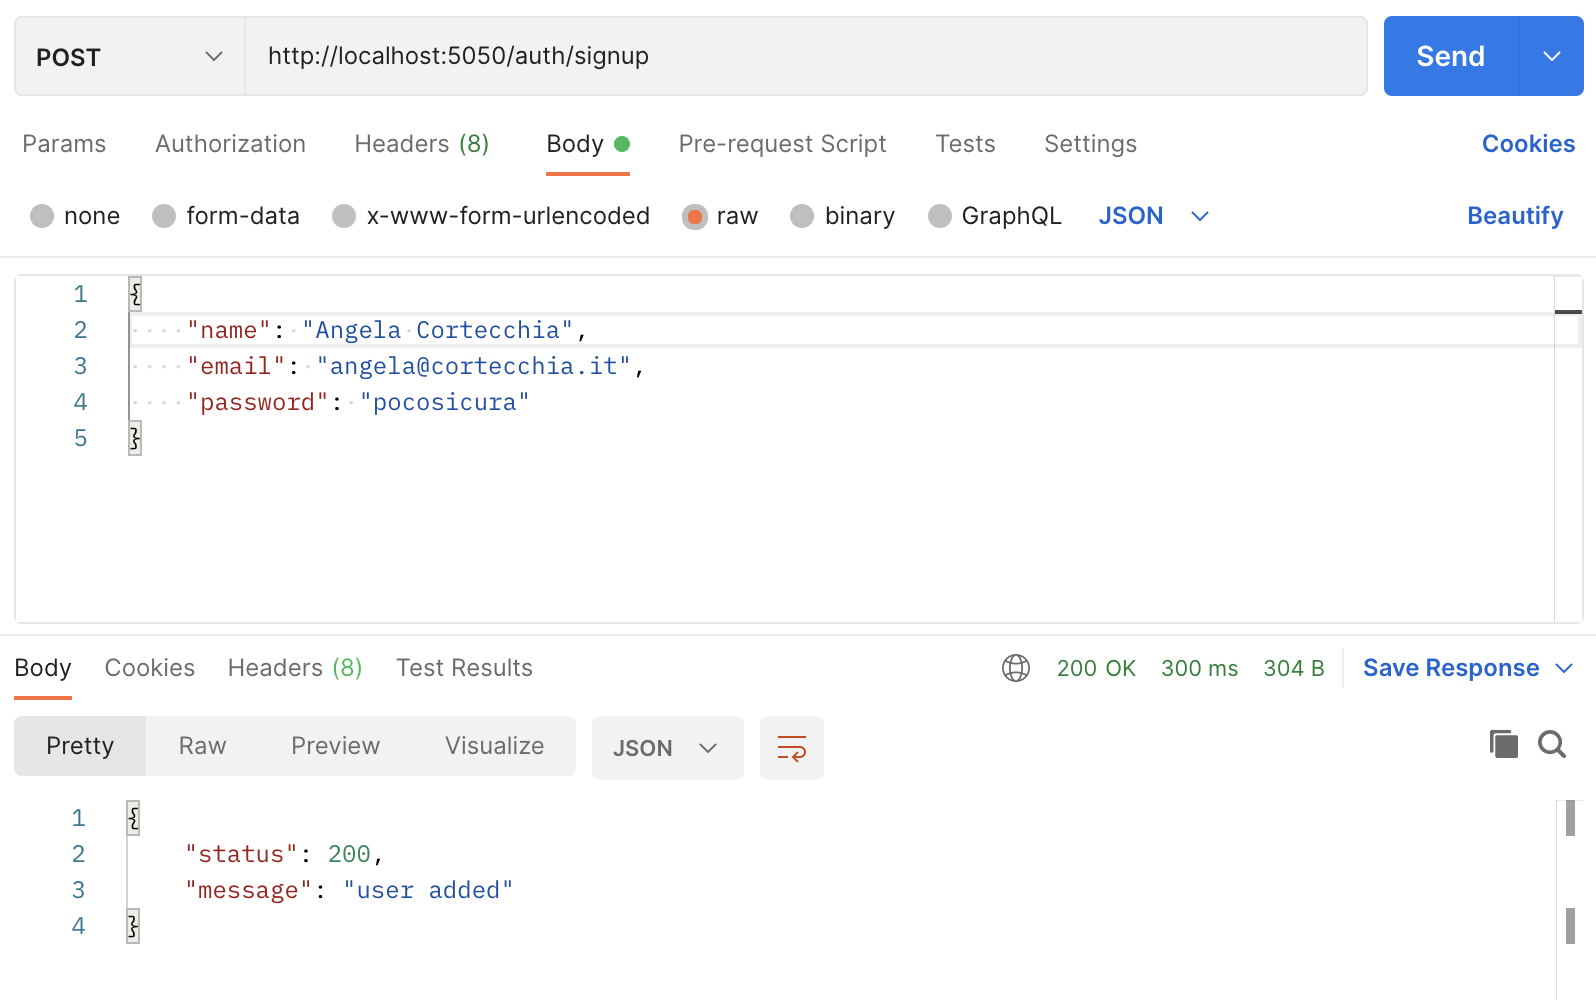
\includegraphics[width=\textwidth]{images/signupPostman.png}
    \caption{Richiesta di registrazione effettuata tramite Postman}
    \label{fig:signupPostman}
\end{figure}

\begin{figure}[htbp]
    \centering
    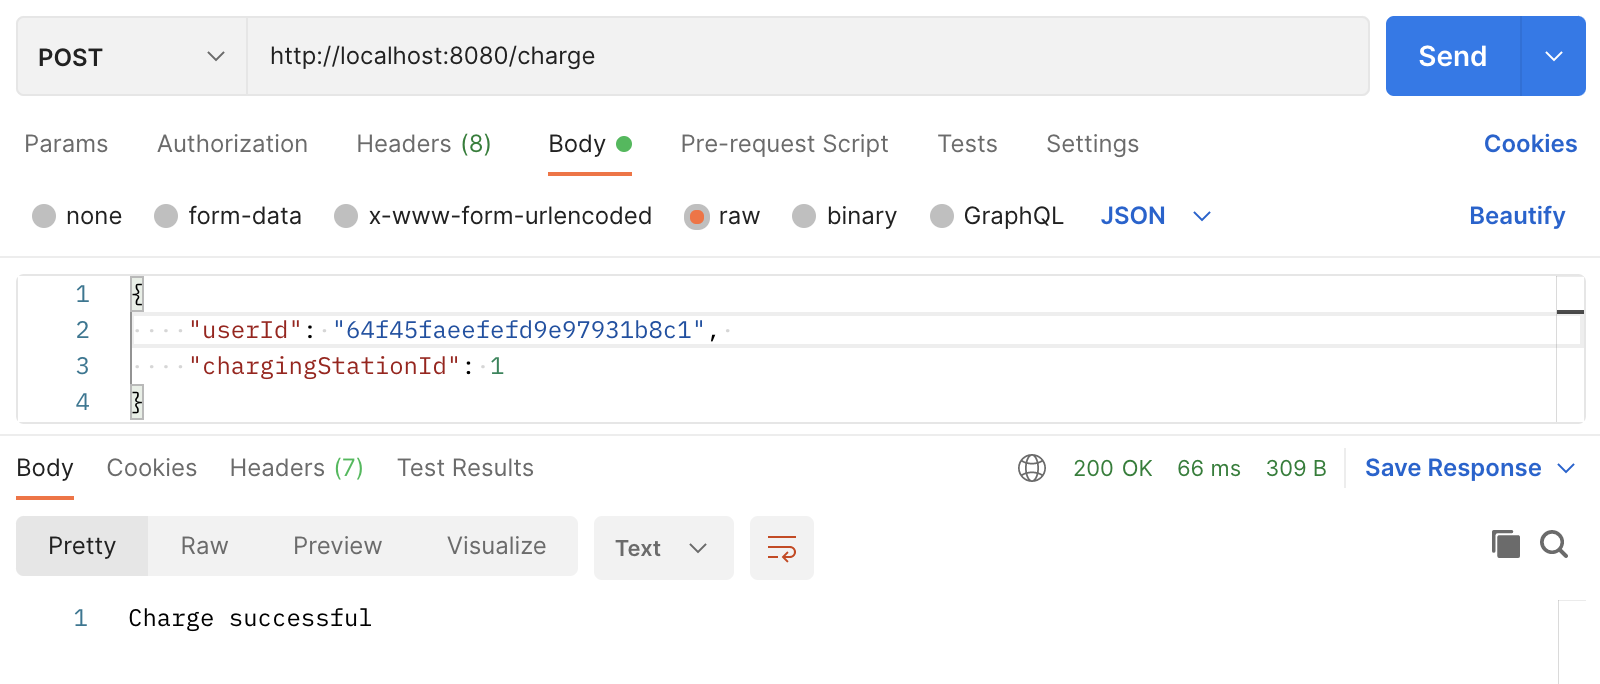
\includegraphics[width=\textwidth]{images/askCharge.png}
    \caption{Richiesta di ricarica presso una colonnina}
    \label{fig:askCharge}
\end{figure}

\begin{figure}[htbp]
    \centering
    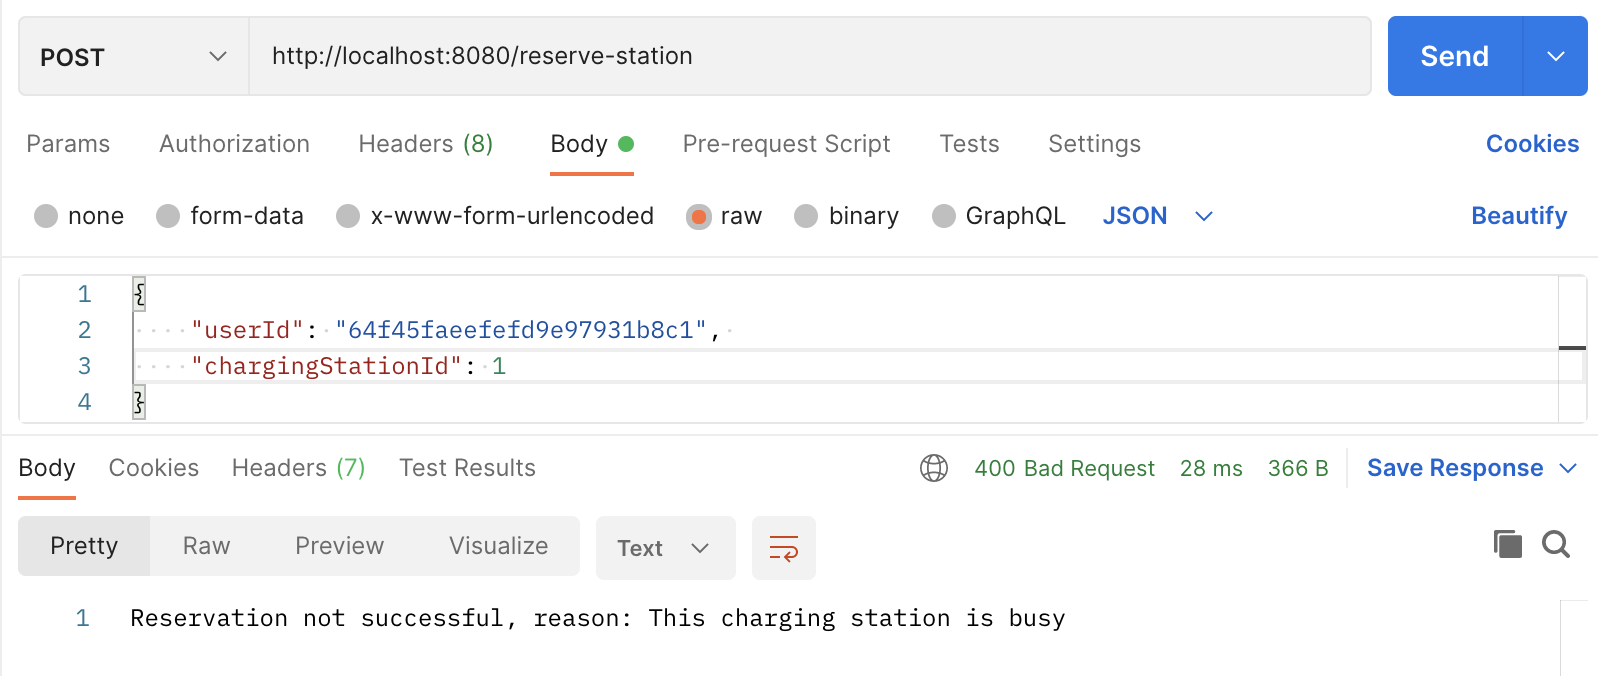
\includegraphics[width=\textwidth]{images/reserveNotOk.png}
    \caption{Richiesta di prenotazione di una colonnina non disponibile}
    \label{fig:reserveNotOk}
\end{figure}

\subsection{Charging Station Domain}
\subsubsection{Unit Testing}
\subsubsection{Integration Testing}

\subsection{User Domain}

Esporre lo stato di funzionamento effettivo del sistema progettato ad elaborato concluso. Per ciascuna delle funzionalità salienti devono essere tabellate e discusse le performance riscontrate mediante opportuni test eseguiti in fase di validazione del progetto.\\

I tempi di esecuzione/comunicazione devono essere accompagnati dalle caratteristiche dell'hardware sul quale è eseguito il software.\\


Vincoli circa la lunghezza della sezione (escluse didascalie, tabelle, testo nelle immagini, schemi):

\vspace{1cm}
\begin{tabular}{l|rr}
                 & Numero minimo di battute & Numero massimo di battute \\
    \hline
    1 componente & 2000                     & 3000                      \\
    2 componenti & 2500                     & 4500                      \\
    3 componenti & 3000                     & 6000                      \\
    \hline
\end{tabular}


\newpage

%----------------------------------------------------------------------------------------
%	ANALISI DI DEPLOYMENT SU LARGA SCALA
%----------------------------------------------------------------------------------------

\section{Analisi di deployment su larga scala}

L'applicativo è stato progettato tenendo in considerazione la possibilità di essere eseguito su larga scala.\\

\subsection{Client App}
Per quanto riguarda il lato client e il server per l'autenticazione sarebbe possibile eseguire il
deployment su cloud tramite servizi come Vercel \cite{vercel}.\\

Grazie alle funzionalità messe a disposizione dal servizio, è possibile mantenere un deploy
continuo dell'applicativo, in modo da poter aggiornare il codice in produzione in maniera
semplice e veloce, tramite semplici push sul main branch di GitHub \cite{github}, grazie all'integrazione del bot offerto da Vercel.\\

\subsection{Database}
Il deployment del database su un cluster di MongoDB Atlas \cite{atlas} ha svolto un ruolo cruciale nel progetto.
Questa soluzione basata su cloud ha permesso di liberarsi dalla gestione dell'infrastruttura, consentendo
di concentrarsi maggiormente sullo sviluppo dell'applicazione stessa. La scalabilità offerta da MongoDB
Atlas ha garantito prestazioni elevate e adattabilità alle crescenti esigenze dell'applicazione.\\

Inoltre, sono stati sfruttati strumenti avanzati per la sicurezza dei dati e il monitoraggio delle attività.
Complessivamente, questa scelta ha contribuito al successo del progetto, garantendo affidabilità e sicurezza.\\

\subsection{Cluster}
Per quanto riguarda invece il lato "cluster" del sistema, il gruppo ha immaginato di effettuare
il deployment dei ChargingStationActor direttamente nelle stazioni di ricarica, mentre i
componenti Charging Station Provider e Service possono essere deployati su nodi fisicamente
separati dalle stazioni di ricarica. Akka cluster permette al sistema di aggiungere facilmente
nuovi attori di qualunque tipo per soddisfare le esigenze di scalabilità del sistema.\\

Il deployment finale così come immaginato dal gruppo è rappresentato dal seguente diagramma \ref{fig:deployment}:

\begin{figure}[H]
    \centering
    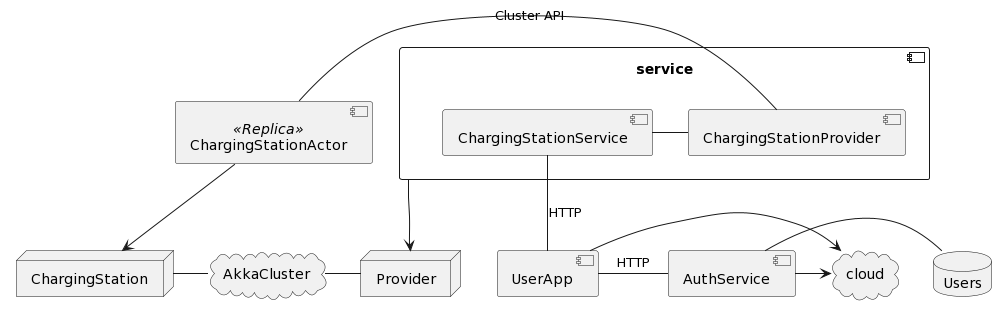
\includegraphics[width=1\textwidth]{images/deployment.png}
    \caption{Diagramma di deployment}
    \label{fig:deployment}
\end{figure}

% In questa sezione va discussa, eventualmente con l'ausilio di opportuni diagrammi (componenti, deployment), l'evoluzione del progetto presentato immaginando che venga adottato su larga scala. I dettagli qui esposti devono quindi astrarre dalle specifiche dell'elaborato qualora l'implementazione sia stata focalizzata su uno scenario isolato.\\

% A titolo d’esempio, qualora applicabile, devono essere evidenziate le criticità che si potrebbero incontrare e devono essere proposte soluzioni tipiche in contesti di \textit{cloud architecture} per garantire un'adeguata \textit{resilienza}, in termini di \textit{availability} e \textit{scalability} del sistema.\\


% Vincoli circa la lunghezza della sezione (escluse didascalie, tabelle, testo nelle immagini, schemi):

% \vspace{1cm}
% \begin{tabular}{l|rr}
%                  & Numero minimo di battute & Numero massimo di battute \\
%     \hline
%     1 componente & 3000                     & 6000                      \\
%     2 componenti & 4500                     & 9000                      \\
%     3 componenti & 6000                     & 12000                     \\
%     \hline
% \end{tabular}


\newpage


%----------------------------------------------------------------------------------------
%	PIANO DI LAVORO
%----------------------------------------------------------------------------------------

\section{Piano di lavoro}
È stata concordata l'adozione di un approccio allo sviluppo ispirato alle
metodologie agili, con sprint settimanali. Gli sprint settimanali sono stati pianificati in incontri di sprint planning, durante i quali veniva definito il lavoro da svolgere per la settimana successiva. Questo lavoro veniva equamente suddiviso tra i membri del team, tenendo conto delle competenze e delle risorse disponibili.


A questi incontri sono state aggiunte retrospettive
per ogni sprint per fare il punto sullo stato di completamento del lavoro pianificato.\\

Inizialmente, è stato condotto uno studio approfondito sulle tecnologie disponibili e sullo stato attuale delle conoscenze nel settore. Questo studio ha permesso di prendere decisioni informate sulla scelta delle tecnologie da utilizzare e di adottare le metodologie più avanzate e adatte al contesto di sviluppo.\\

In seguito, è stato pianificato il lavoro da svolgere per ogni sprint, tenendo conto
delle risorse disponibili e delle priorità.\\


\subsection{Metodologia adottata}
Un elemento chiave di questa metodologia è stata l'aggiunta delle retrospettive alla fine di ogni sprint. Queste retrospettive hanno permesso al team di fare il punto sullo stato di completamento del lavoro pianificato e di identificare eventuali aree di miglioramento. Questo ciclo di feedback continuo ha contribuito a ottimizzare il processo di sviluppo e a garantire una progressiva evoluzione del progetto.

L'adozione di un approccio agile con sprint settimanali ha consentito al team di sviluppo di mantenere un alto grado di flessibilità, di adattarsi rapidamente ai cambiamenti e di garantire una progressiva evoluzione del progetto, il tutto basato su uno studio approfondito delle tecnologie e delle metodologie disponibili.

\subsubsection{Sprints}

\begin{itemize}
    \item Sprint 1
          \begin{itemize}

              \item Studio comportamento ideale del sistema ad attori (Cortecchia e Micelli - 1 giorno uomo a testa)
              \item Setup CI/CD (Micelli - 1.5 giorni uomo)
              \item Setup tests (Micelli - 1 giorno uomo)
              \item Implementazione dell'attore inerente alla colonnina di ricarica e relativi test (Cortecchia - 2 giorni uomo a testa)
              \item Implementazione dell'attore inerente alla macchina e relativi test (Micelli - 2 giorni uomo)
          \end{itemize}

    \item Sprint 2
          \begin{itemize}
              \item Studio del framework Svelte (Cortecchia - 1 giorno uomo)
              \item Implementazione di una prima versione della web app (Cortecchia - 2 giorni uomo)
              \item Implementazione dei servizi REST (e relativo studio) lato colonnine (Micelli - 2.5 giorni uomo)
          \end{itemize}

    \item Sprint 3
          \begin{itemize}

              \item Integrazione del servizio di mappe e geolocalizzazione (Cortecchia - 2.5 giorni uomo)
              \item Integrazione del servizio di scanning QR code (Cortecchia - 1 giorni uomo)
              \item Utilizzo di Akka Cluster per i servizi delle colonnine di ricarica (Micelli - 2 giorni uomo)
              \item Refactoring e rimozione degli attori inerenti alle macchine (Micelli - 1 giorno uomo)

          \end{itemize}
    \item Sprint 4
          \begin{itemize}
              \item Implementazione web server express (Cortecchia - 1 giorno uomo)
              \item Configurazione database MongoDB (Cortecchia - 0.5 giorno uomo)
              \item Implementazione dei servizi di autenticazione (Cortecchia - 1 giorno uomo)
              \item Implementazione Akka HTTP per la comunicazione con webapp (Micelli - 3 giorni uomo)
          \end{itemize}
\end{itemize}

\subsection{DevOps}
Per quanto riguarda il processo di sviluppo, il gruppo ha adottato alcune tecniche di DevOps per migliorare la qualità del software e la produttività del team.\\
La prima scelta fatta è stata la suddivisione del progetto in varie repositories indipendenti. Ciascuna di queste repository è stata gestita secondo le seguenti modalità:

\begin{itemize}
    \item \textbf{Branching model}: è stato adottato un branching model ispirato al GitFlow, con un branch main per il codice in produzione e vari feature branch per lo sviluppo di nuove funzionalità. Questo approccio ha permesso di mantenere un alto grado di flessibilità e di adattarsi rapidamente ai cambiamenti.
    \item \textbf{Pull request}: ogni modifica al codice è stata effettuata tramite pull request. Questo approccio ha permesso di proteggere al meglio il main branch da modifiche non testate e di sfruttare al meglio la Continuous Integration.
    \item \textbf{Continuous Integration}: è stato configurato un sistema di Continuous Integration per ogni repository grazie al meccanismo delle Github Actions. In particolare è stato creato un workflow che eseguiva il setup di vari ambienti di esecuzione e che eseguiva i test specificati.
\end{itemize}


% In questa sezione devono essere chiariti i compiti svolti da ciascun candidato nel caso in cui il gruppo abbia più di un componente.\\

% Deve essere inoltre esposto il piano di lavoro adottato. A tal fine, per ogni attività svolta durante la preparazione dell'elaborato (ad esempio: studio di una tecnologia, progettazione di un componente, implementazione di un algoritmo ecc…) deve essere chiarita la collocazione temporale e devono essere indicate le risorse impiegate per svolgerla (giorni/uomo). I candidati possono ricorrere a opportuni diagrammi come quello di Gantt.\\


% Vincoli circa la lunghezza della sezione (escluse didascalie, tabelle, testo nelle immagini, schemi):

% \vspace{1cm}
% \begin{tabular}{l|rr}
%  & Numero minimo di battute & Numero massimo di battute \\
%  \hline
%  1 componente & 1000 & 2000 \\
%  2 componenti & 1500 & 3000 \\
%  3 componenti & 2000 & 4000 \\
%  \hline
% \end{tabular}

\newpage




% \begin{tabular}{l|rr}
%  ID Sprint & Attività & Assegnati & Tempistica (gg uomo)
%  \hline
%  1 & Studio colonnine; visualizzazione stato colonnina & Cortecchia, Micelli & xxx
%  \hline
% \end{tabular}





%----------------------------------------------------------------------------------------
%	CONCLUSIONI
%----------------------------------------------------------------------------------------

\section{Conclusioni}

Nel corso di questo progetto, ci siamo impegnati a sviluppare un'applicazione innovativa per
la gestione delle colonnine di ricarica in ambito smart city. Le nostre conclusioni riflettono
l'importanza fondamentale di tale iniziativa nell'accelerare la transizione verso città più
sostenibili ed efficienti dal punto di vista energetico.

In primo luogo, abbiamo constatato che l'applicazione ha il potenziale per migliorare la
gestione delle colonnine di ricarica, consentendo controllo e supervisione
continui. Questo si traduce in una maggiore affidabilità e disponibilità delle infrastrutture
di ricarica, migliorando l'esperienza dell'utente finale e incoraggiando l'adozione di veicoli
elettrici. Inoltre, l'ottimizzazione della gestione delle colonnine può contribuire a ridurre
i costi operativi e a massimizzare l'efficienza energetica, promuovendo al contempo una riduzione
delle emissioni nocive.

Le nostre considerazioni indicano che l'applicazione può essere facilmente adattata per soddisfare
le esigenze specifiche di diverse città e comunità, favorendo così l'espansione del nostro progetto
in molteplici contesti urbani. Inoltre, è importante sottolineare il potenziale impatto positivo sulla
mobilità e sull'ambiente. L'uso diffuso di veicoli elettrici ridurrà notevolmente le emissioni di gas
serra e l'inquinamento atmosferico, contribuendo a combattere i cambiamenti climatici e a migliorare
la qualità dell'aria nelle città.

Tuttavia, è necessario considerare alcune sfide e questioni critiche per il successo continuo
del progetto. In primo luogo, è fondamentale garantire la sicurezza delle infrastrutture e dei
dati associati all'applicazione, proteggendoli da potenziali minacce informatiche. Inoltre,
è importante coinvolgere attivamente le autorità locali, gli operatori di rete e gli stakeholder
interessati per promuovere una collaborazione efficace e garantire l'adozione diffusa dell'applicazione.

In conclusione, il nostro progetto ha dimostrato il potenziale di un'applicazione per
la gestione delle colonnine di ricarica nell'ambito delle smart city. Le opportunità di
miglioramento dell'efficienza energetica, la promozione dei veicoli elettrici e la riduzione
delle emissioni di gas serra sono tutti obiettivi che meritano di essere perseguiti con
determinazione. Con il giusto impegno e collaborazione, possiamo contribuire in modo
significativo a creare città più sostenibili e abitabili per le future generazioni.

\subsection{Sviluppi futuri}

Per quanto riguardan l'applicazione lato client, possono essere identificati i seguenti sviluppi futuri:

\begin{itemize}
    \item Possibilità di effettuare pagamenti in-app attraverso l'integrazione di servizi di terze parti;
    \item Filtraggio nella visualizzazione delle colonnine in base alle caratteristiche della macchina;
    \item Integrazione con altre app per la gestione della mobilità urbana;
    \item Integrazione con app dedicate alla navigazione, per gestire itinerari che includono soste per la ricarica.
\end{itemize}

Invece, per quanto riguarda il lato "cluster" del sistema, il gruppo ha identificato i seguenti possibili sviluppi futuri:

\begin{itemize}
    \item Esplorazione di una soluzione per includere l'applicativo client all'interno del cluster akka, in modo da farla comunicare in maniera peer-to-peer con le stazioni di ricarica;
    \item Esposizione all'esterno delle Charging Stations attraverso Akka Stream ed il protocollo WebSocket, per permettere ai client web di osservare lo stato delle stazioni in tempo reale;
    \item Generalizzazione dell'architettura per supportare altri tipi di dispositivi e servizi in ambito smart city;
\end{itemize}

\newpage

\bibliographystyle{plain}
\addcontentsline{toc}{section}{Riferimenti bibliografici}

\bibliography{bibliography}

\end{document}